%%%%%%%%%%%%%%%%%%%%%%%%%%%%%%%%%%%%%%%%%
% University/School Laboratory Report
% LaTeX Template
% Version 3.1 (25/3/14)
%
% This template has been downloaded from:
% http://www.LaTeXTemplates.com
%
% Original author:
% Linux and Unix Users Group at Virginia Tech Wiki 
% (https://vtluug.org/wiki/Example_LaTeX_chem_lab_report)
%
% License:
% CC BY-NC-SA 3.0 (http://creativecommons.org/licenses/by-nc-sa/3.0/)
%
%%%%%%%%%%%%%%%%%%%%%%%%%%%%%%%%%%%%%%%%%

%----------------------------------------------------------------------------------------
%	PACKAGES AND DOCUMENT CONFIGURATIONS
%----------------------------------------------------------------------------------------

\documentclass{article}




\usepackage{natbib} % Required to change bibliography style to APA
\usepackage{siunitx}
\usepackage{cite, graphicx, amsmath}
\usepackage{caption}
\usepackage{subcaption}
\setlength\parindent{0pt} % Removes all indentation from paragraphs

\renewcommand{\labelenumi}{\alph{enumi}.} % Make numbering in the enumerate environment by letter rather than number (e.g. section 6)

%\usepackage{times} % Uncomment to use the Times New Roman font

%----------------------------------------------------------------------------------------
%	DOCUMENT INFORMATION
%----------------------------------------------------------------------------------------

\title{Image processing and evaluation of image quality} % Title

\author{\textsc{Federico Battisti - Massimiliano Galli}} % Author name

\date{\today} % Date for the report

\begin{document}

\maketitle % Insert the title, author and date

\begin{center}
\begin{tabular}{l r}
Date Performed: & June 1, 2018 \\ % Date the experiment was performed
Partners: & Federico Battisti \\ % Partner names
& Massimiliano Galli \\
Instructor: & Nicola Lanconelli % Instructor/supervisor
\end{tabular}
\end{center}
\begin{abstract}

	This is a report for the third laboratory session for the Applied Physics course, regarding image manipulation. The experience was structured into four main exercises: 
	\begin{itemize}
		\item For the first exercise we were asked to reduce the noise present into 3 different images using operations both in the spacial and frequency domain, evaluating each time the quality of the pictures before and after the trasformation by means of signal to noise ratio (SNR) performed on a profile and an extended area were the images were as uniform as possible
		\item For the second exercise we had to perform a similar task on an image containing various parallel lines patterns at different frenquencies. Exploiting this peculiarity we were also able to determine the spacial resolution in terms of MTF before and after the application of spacial and FFT noise reduction filters
		\item For the third exercise we were asked to perform a flat-field correction on a mammographic image and evaluate, before and after, the image quality by means of SNR and Contrast-Noise Ratio (CNR)
		\item Finally, using a phantom containing various framed circles at various diameters and levels of contrast, we were asked to calculate the CNR on each detail and graph that value as a function of the thickness of the detail 
		
	\end{itemize}
\end{abstract}
\clearpage 
\section*{Exercise 1}
For the first part of the experience we were given three different pictures affected by different types of noise and artifacts created during acquisition by the acquisition devices themselfs (Figure). We were then asked to perform operations both in the spatial and frequency domain in order to reduce the effect of the artifacts. In each situation we had to then quantitatively verify the quality of the images before and after the operations performed by considering:
\begin{itemize}
 \item A profile on an almost uniform area and evaluating the background value by means of standard deviation from the mean grey level, which were both provided by ImageJ.A profile can be simply defined as a single line of pixels, the grey levels of which can be analyzed using the profile histogram option in ImageJ.
 \item Signal to Noise Ratio (SNR) on an almost uniform extended area , which can be defined as:
 \begin{equation}
 SNR=\frac{signal}{noise}=\frac{mean\ gray\ level}{gray\ level\ standard\ deviation}
 \end{equation}
 once again both the values can be obtained using the ImajeJ options
\end{itemize}
In the spatial domain we decided to use a median filter for Figure 1a, a mean filter for Figure 1b and a gaussian filter for Figure 1c. As for the FFT operations we decided to apply a low-pass filter to all three of the images, in order to cut all the high frequencies from the frequency domain  , since our objective was to reduce noise. The results of these operations can be seen in Figure 1 and 2 respectively, while the profile standard deviation and the SNR for the extended area for each picture and each transformation are are tabled in table.\\
\begin{table}[h]
	\begin {center}
	\begin{tabular}{| l | l | l | l |}
		\hline
		Figure & Operation & $\sigma_{profile}$ & SNR \\ \hline
		1a & raw & 6.78 & 11.12 \\ \hline
		   & median filter & 3.65 & 23.33 \\ \hline 
		   & low-pass filter & 3.65 & 24.60 \\ \hline 
		1b & raw & 7.45 & 10.28 \\ \hline
		& mean filter & 4.90 & 16.54 \\ \hline 
		& low-pass filter & 5.37 & 16.03 \\ \hline 
		1c & raw & 77.97 & 0.77 \\ \hline
		& gaussian filter & 1.78 & 35.28 \\ \hline 
		& low-pass filter & 7.86 & 5.45 \\ \hline 
	\end{tabular}
	\caption{}
	\end{center}
\end{table}
\\As it was to be expected the noise reduction operations managed to reduce the profile standard deviation and augment the SNR which are are both signs of improvement in image quality.

\begin{figure}[h]
\centering
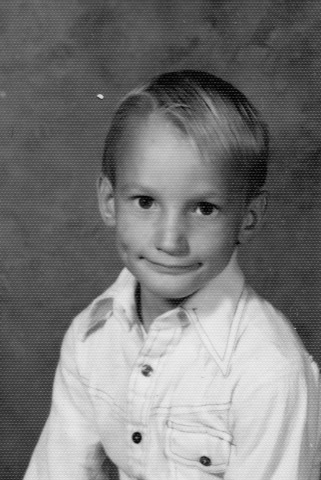
\includegraphics[width=.4\textwidth]{./immagini_terza_prova/kiddo.png}
\bigbreak
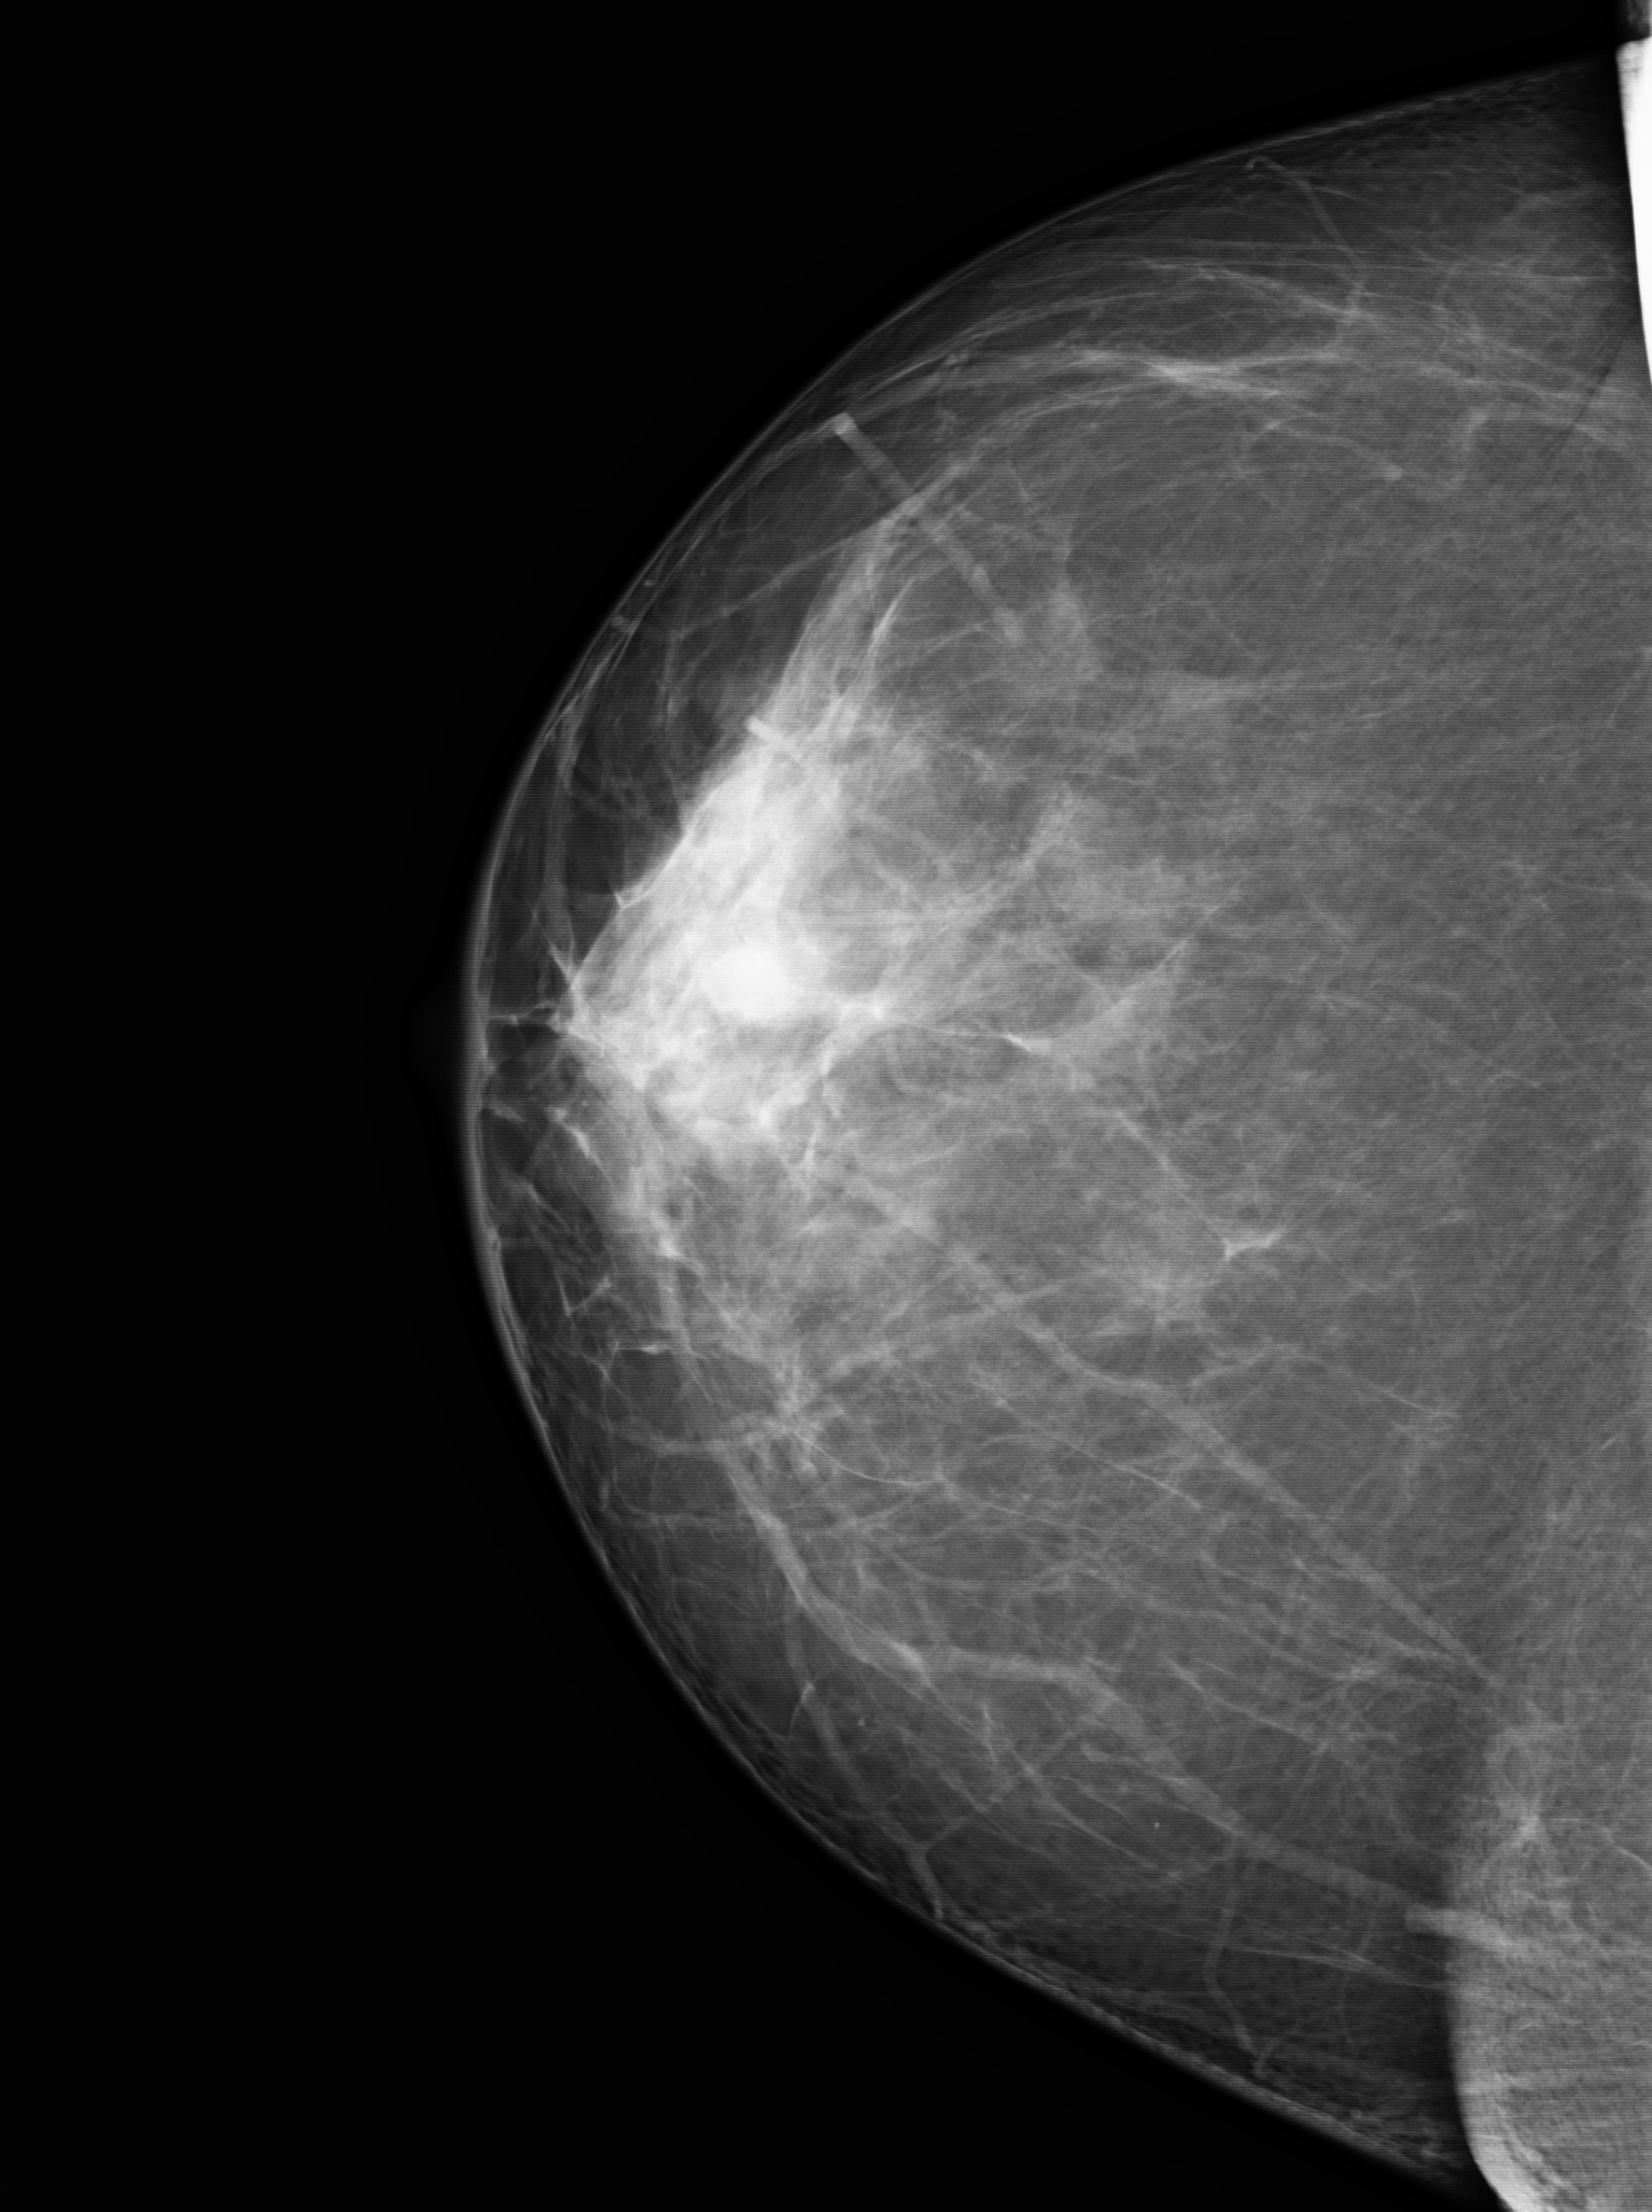
\includegraphics[width=.4\textwidth]{./immagini_terza_prova/griglia_mammo.png}
\bigbreak
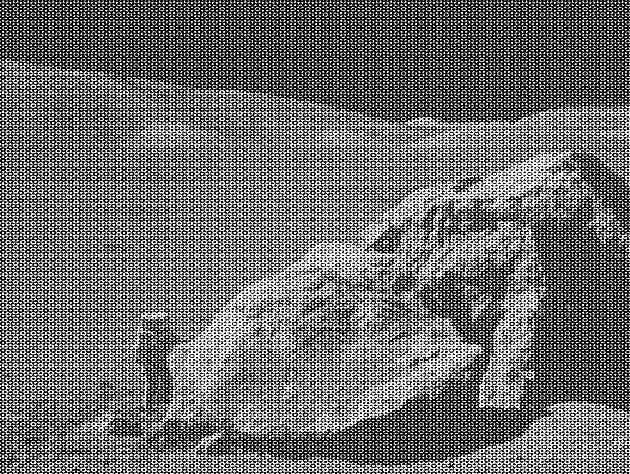
\includegraphics[width=.4\textwidth]{./immagini_terza_prova/moonlanding.png}
\caption{Pictures used in their raw form.(From top to bottom) a, b and c}\label{two}
\end{figure}

\begin{figure}[h]
	\centering
	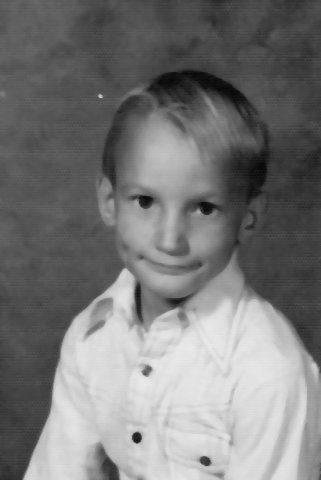
\includegraphics[width=.4\textwidth]{./immagini_terza_prova/kiddo_1/kiddo_median.jpg}
	\bigbreak
	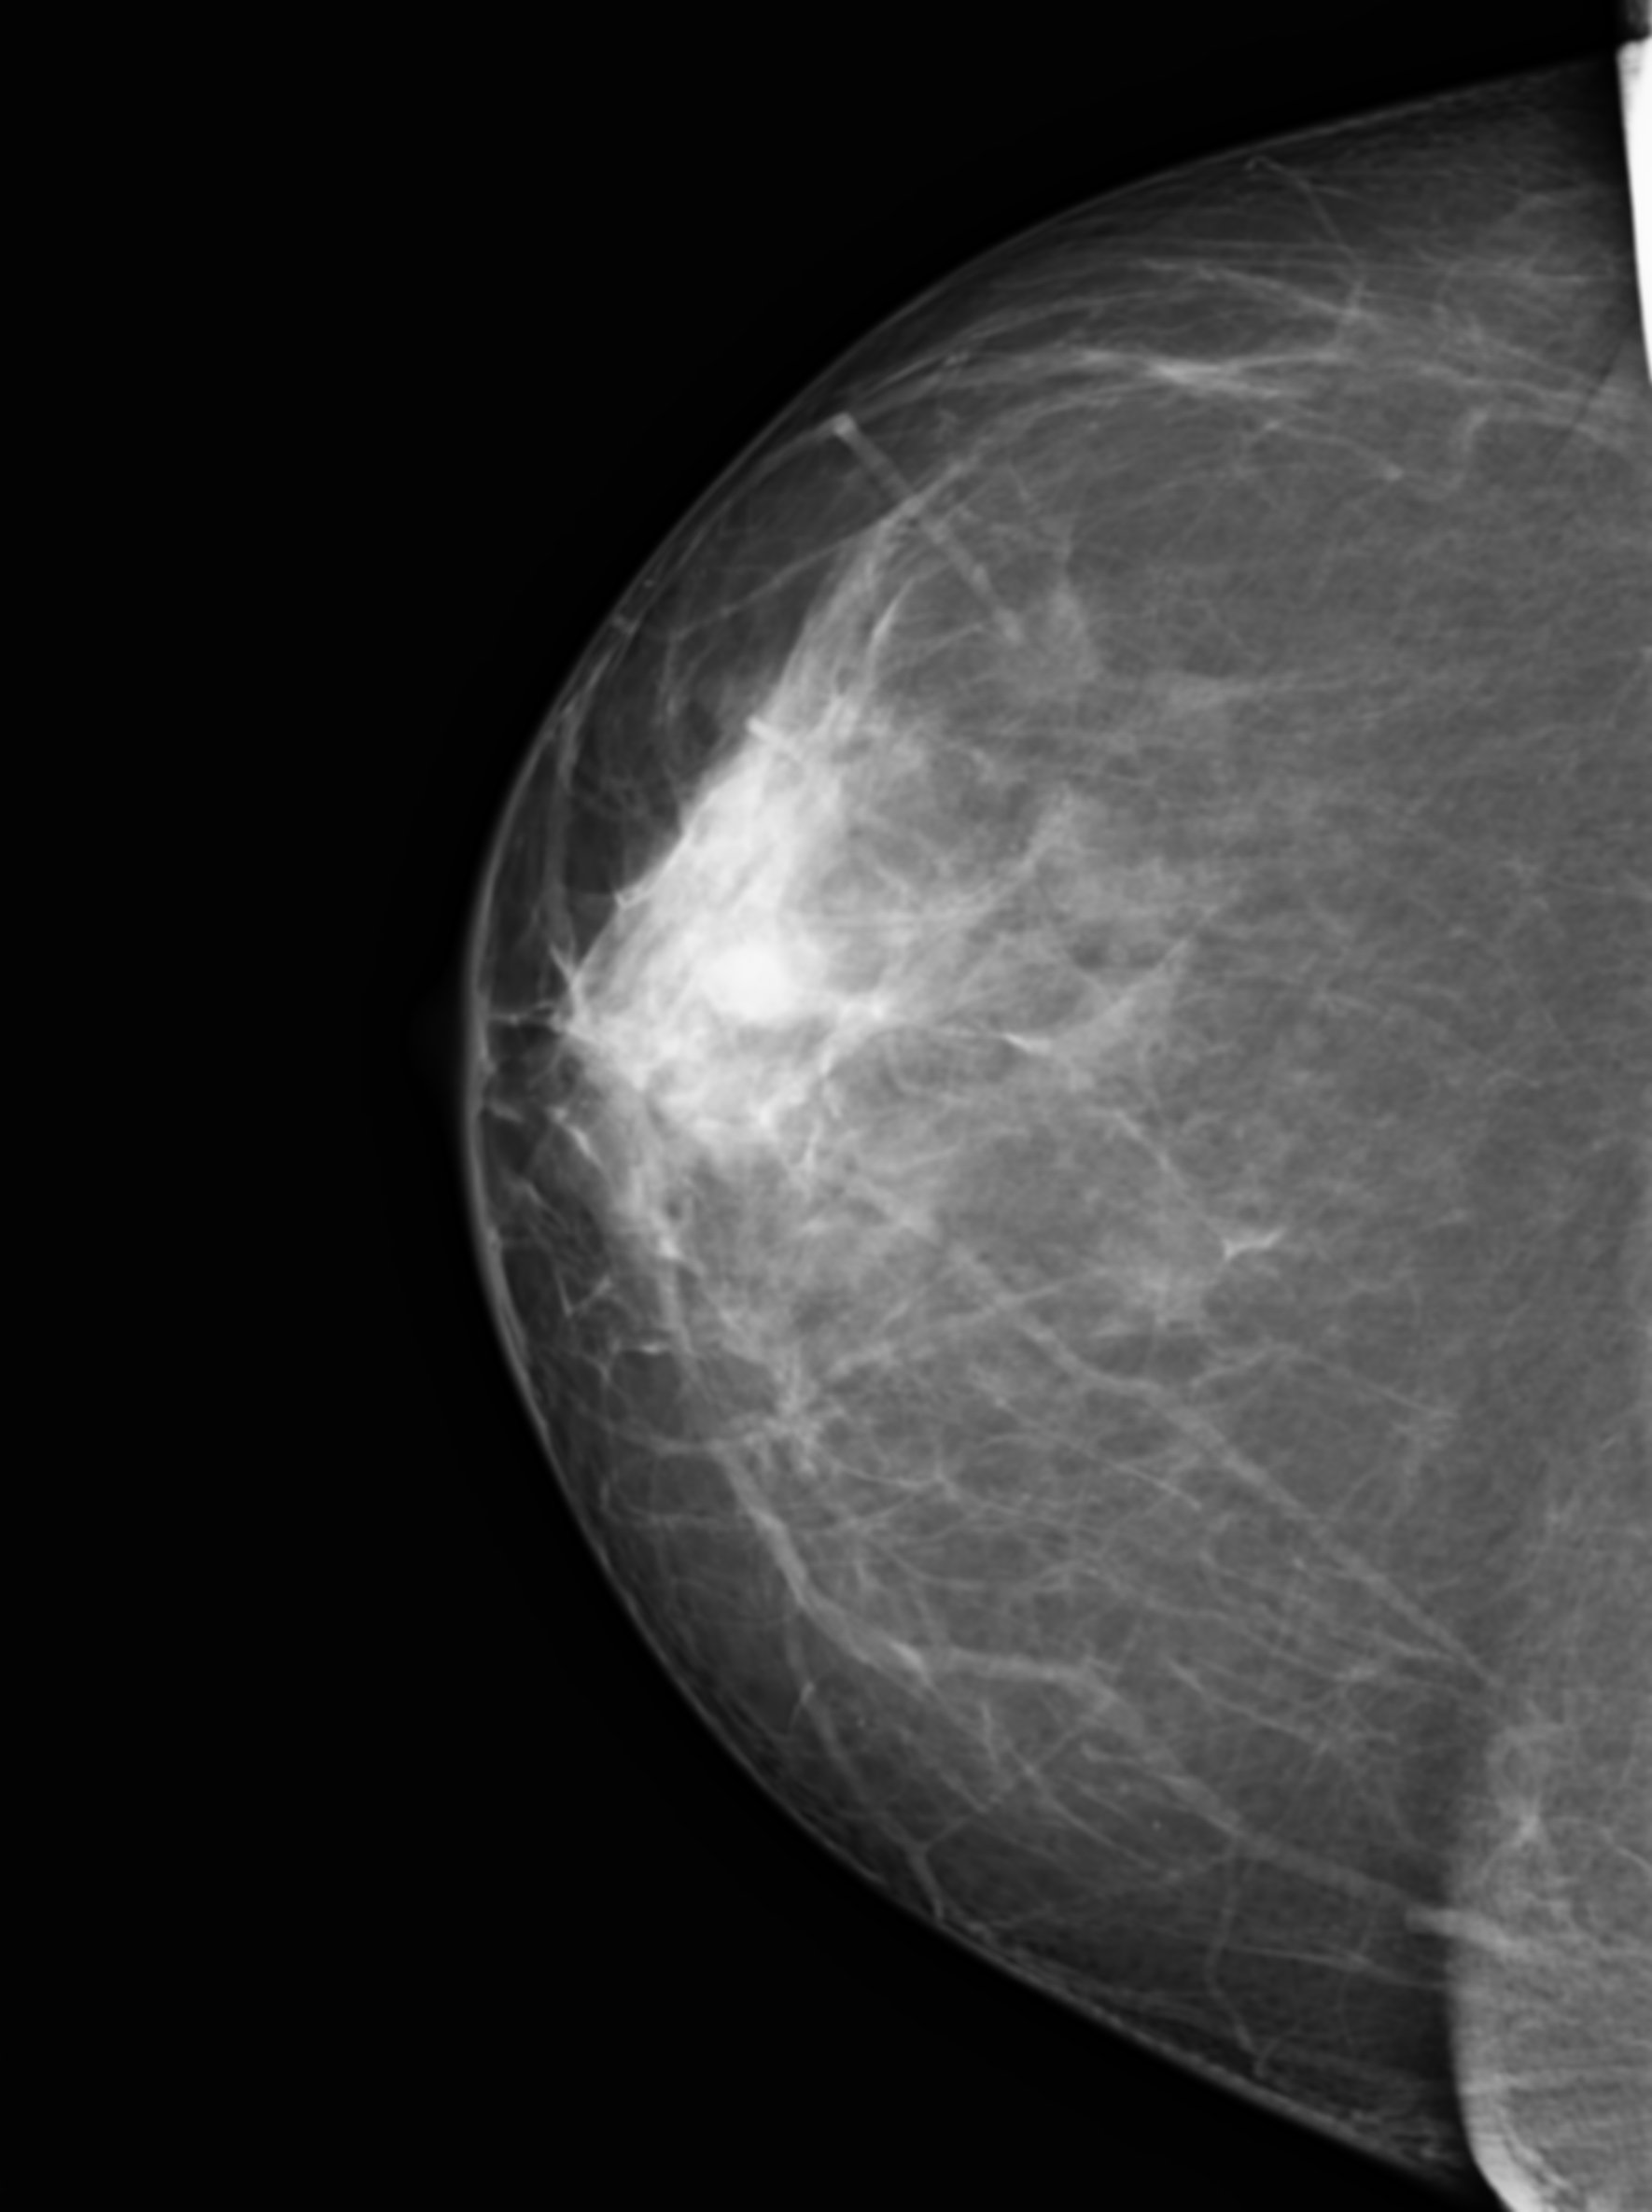
\includegraphics[width=.4\textwidth]{./immagini_terza_prova/tetta_1/tetta_mean.jpg}
	\bigbreak
	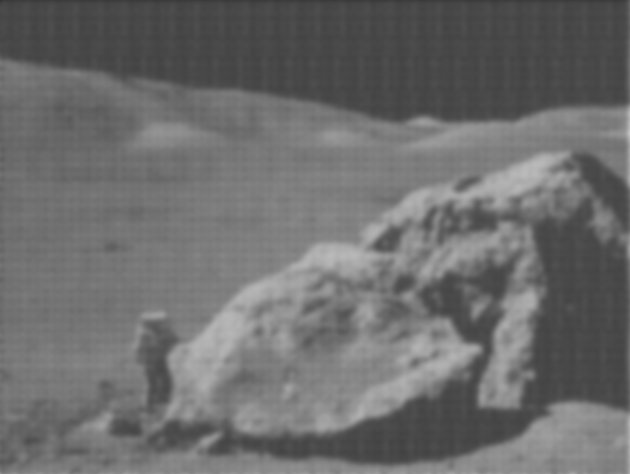
\includegraphics[width=.4\textwidth]{./immagini_terza_prova/moon_1/moonlanding_gauss.jpg}
	\caption{Pictures modified using spatial filters.(From top to bottom) a: median filter; b: mean filter ; c: gaussian filter}\label{two}
\end{figure}
\begin{figure}[h]
	\centering
	\begin{subfigure}[b]{0.5\textwidth}
		\centering
		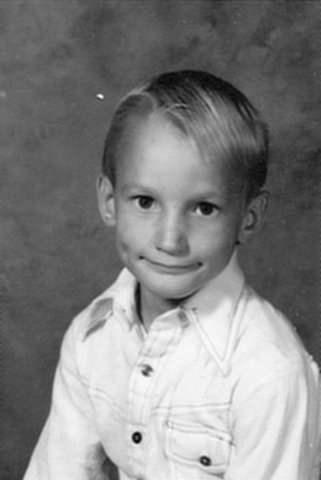
\includegraphics[height=2in]{./immagini_terza_prova/kiddo_1/kiddo_filtered_fft.jpg}
		
	\end{subfigure}%
	\begin{subfigure}[b]{0.5\textwidth}
		\centering
		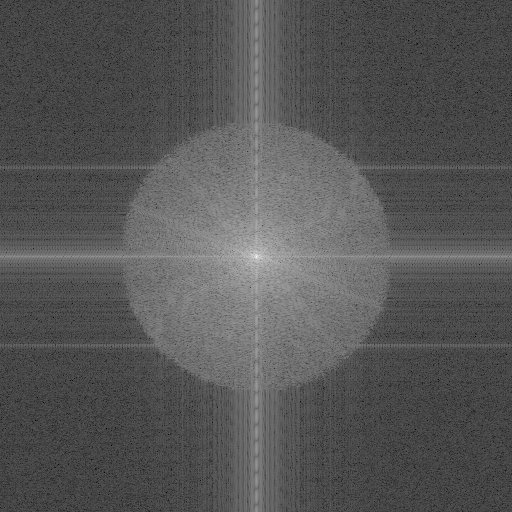
\includegraphics[height=2in]{./immagini_terza_prova/kiddo_1/FFTofkiddo_filtered_fft.jpg}
	
	\end{subfigure}%
	\bigbreak
	
%%%%%%%%%%%%%%%%%%%%%%%%%%%%%%%

\begin{subfigure}[b]{0.5\textwidth}
	\centering
	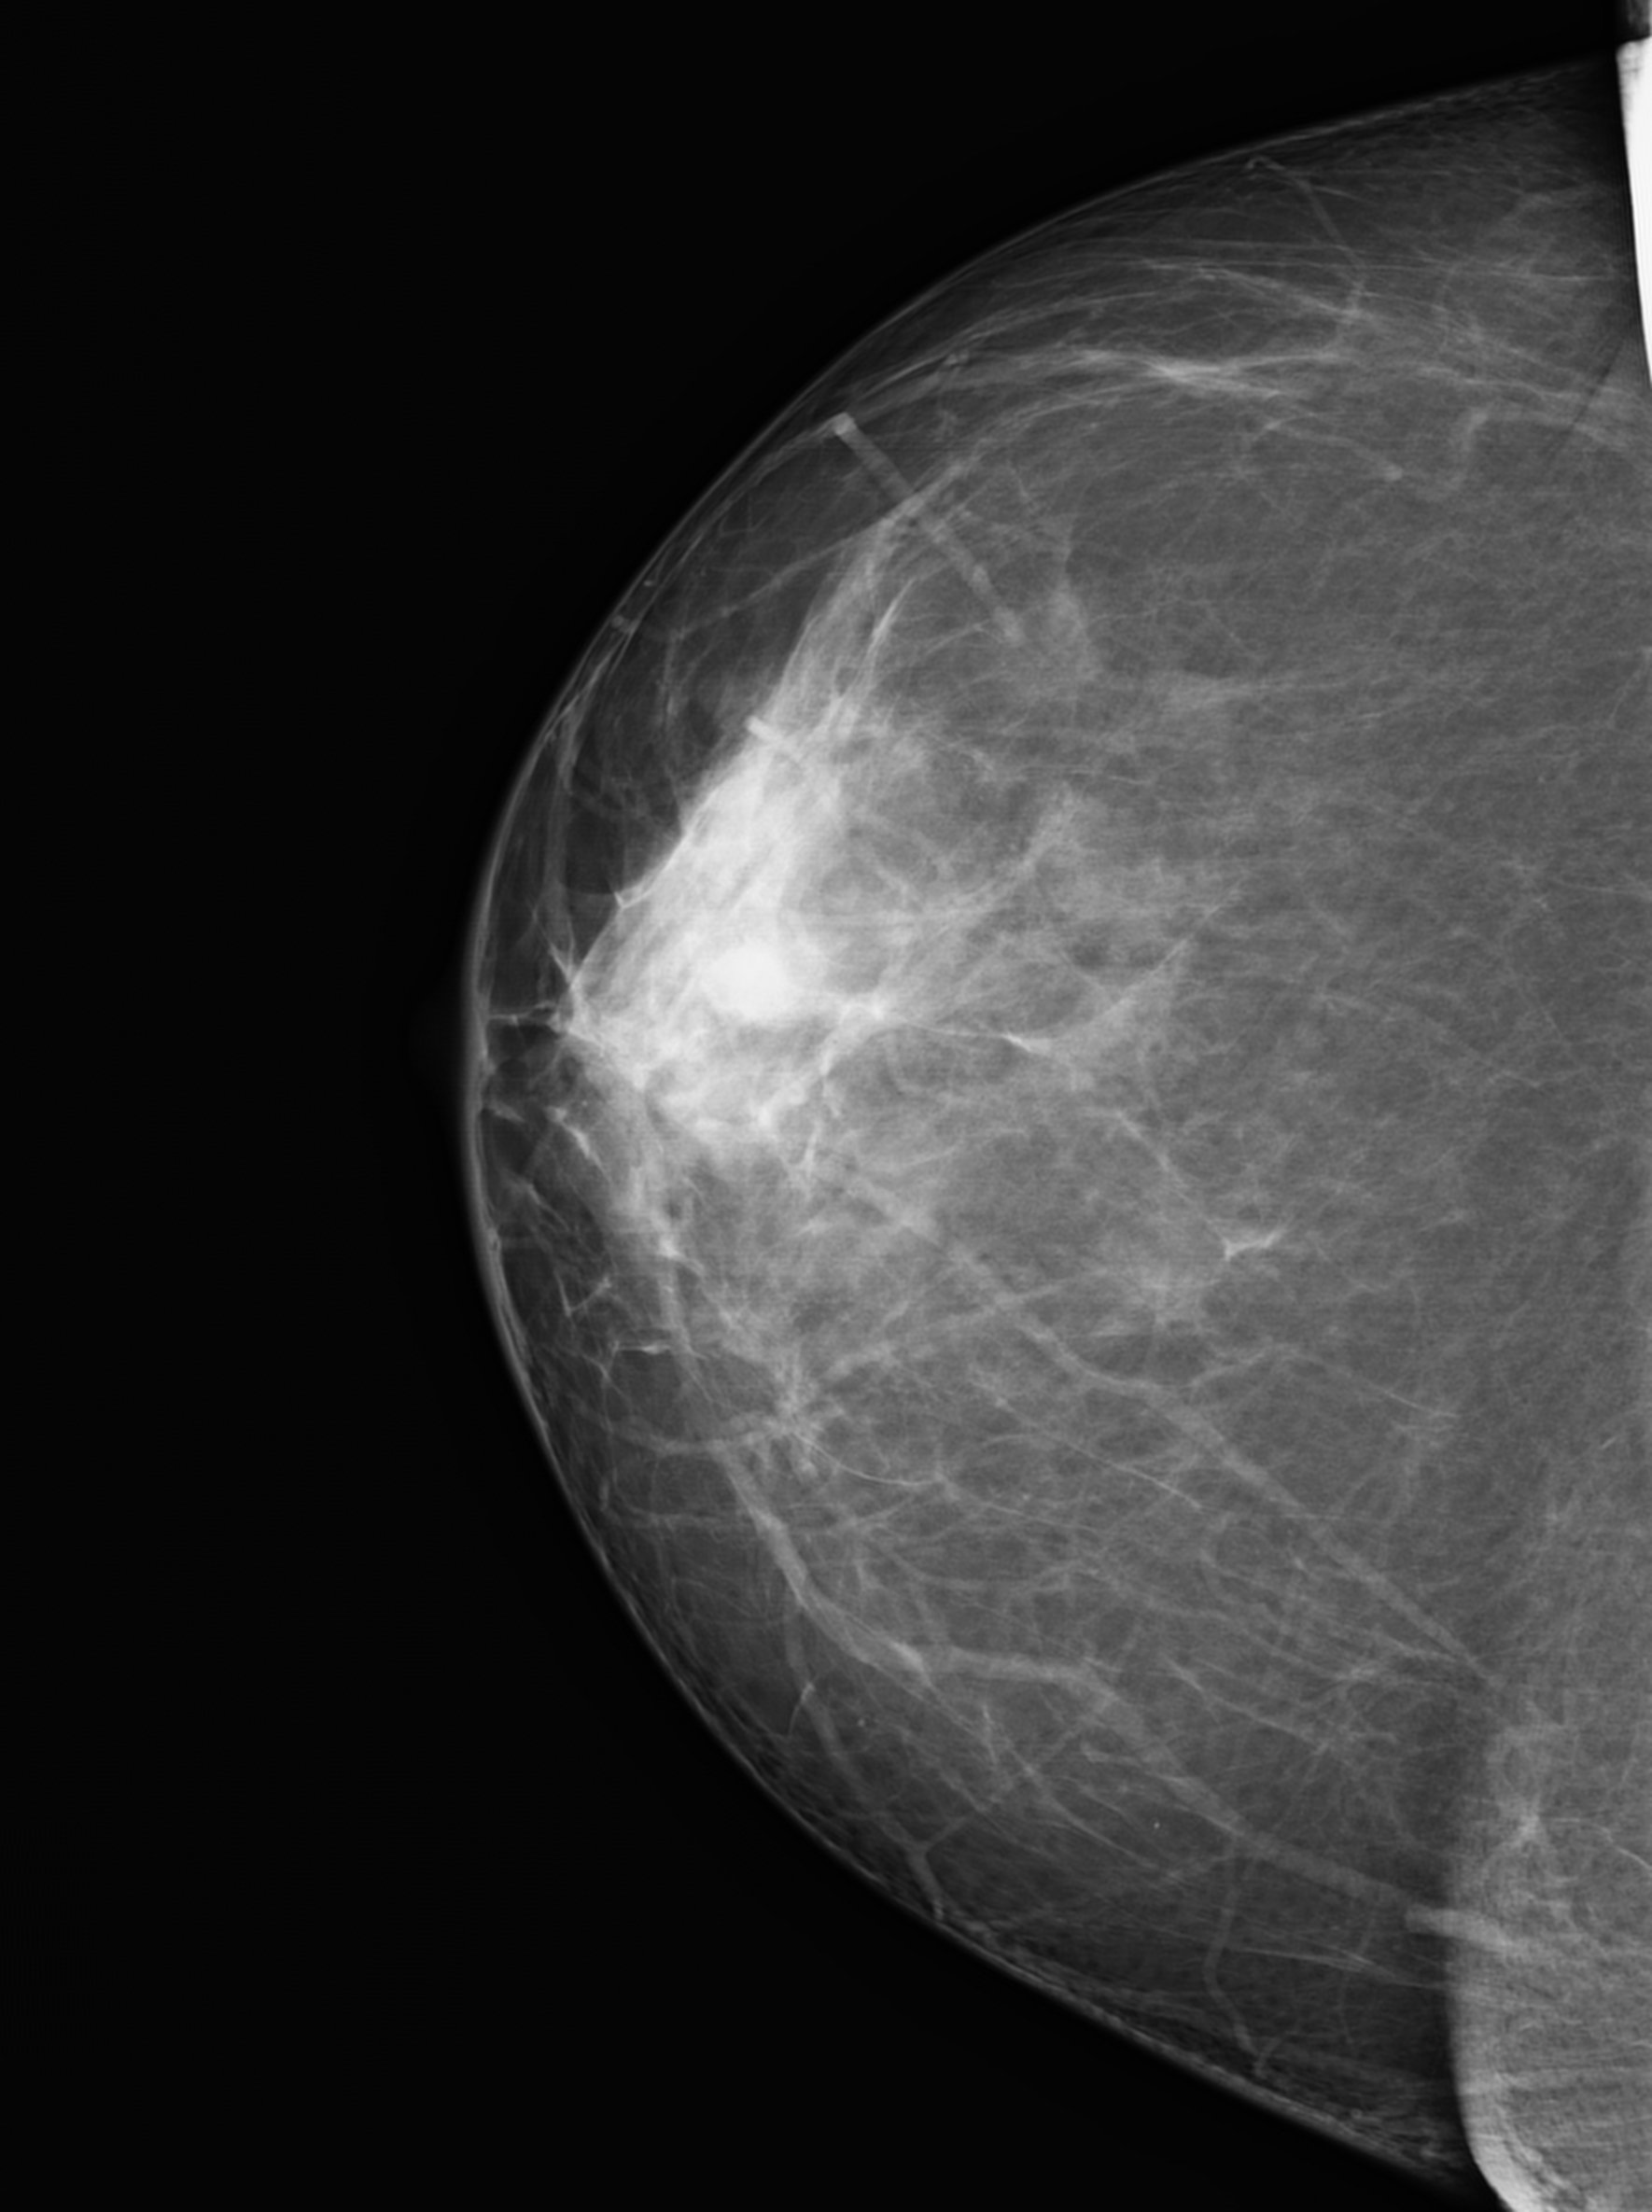
\includegraphics[height=2in]{./immagini_terza_prova/tetta_1/griglia_mammo_fft.jpg}
	
\end{subfigure}%
\begin{subfigure}[b]{0.5\textwidth}
	\centering
	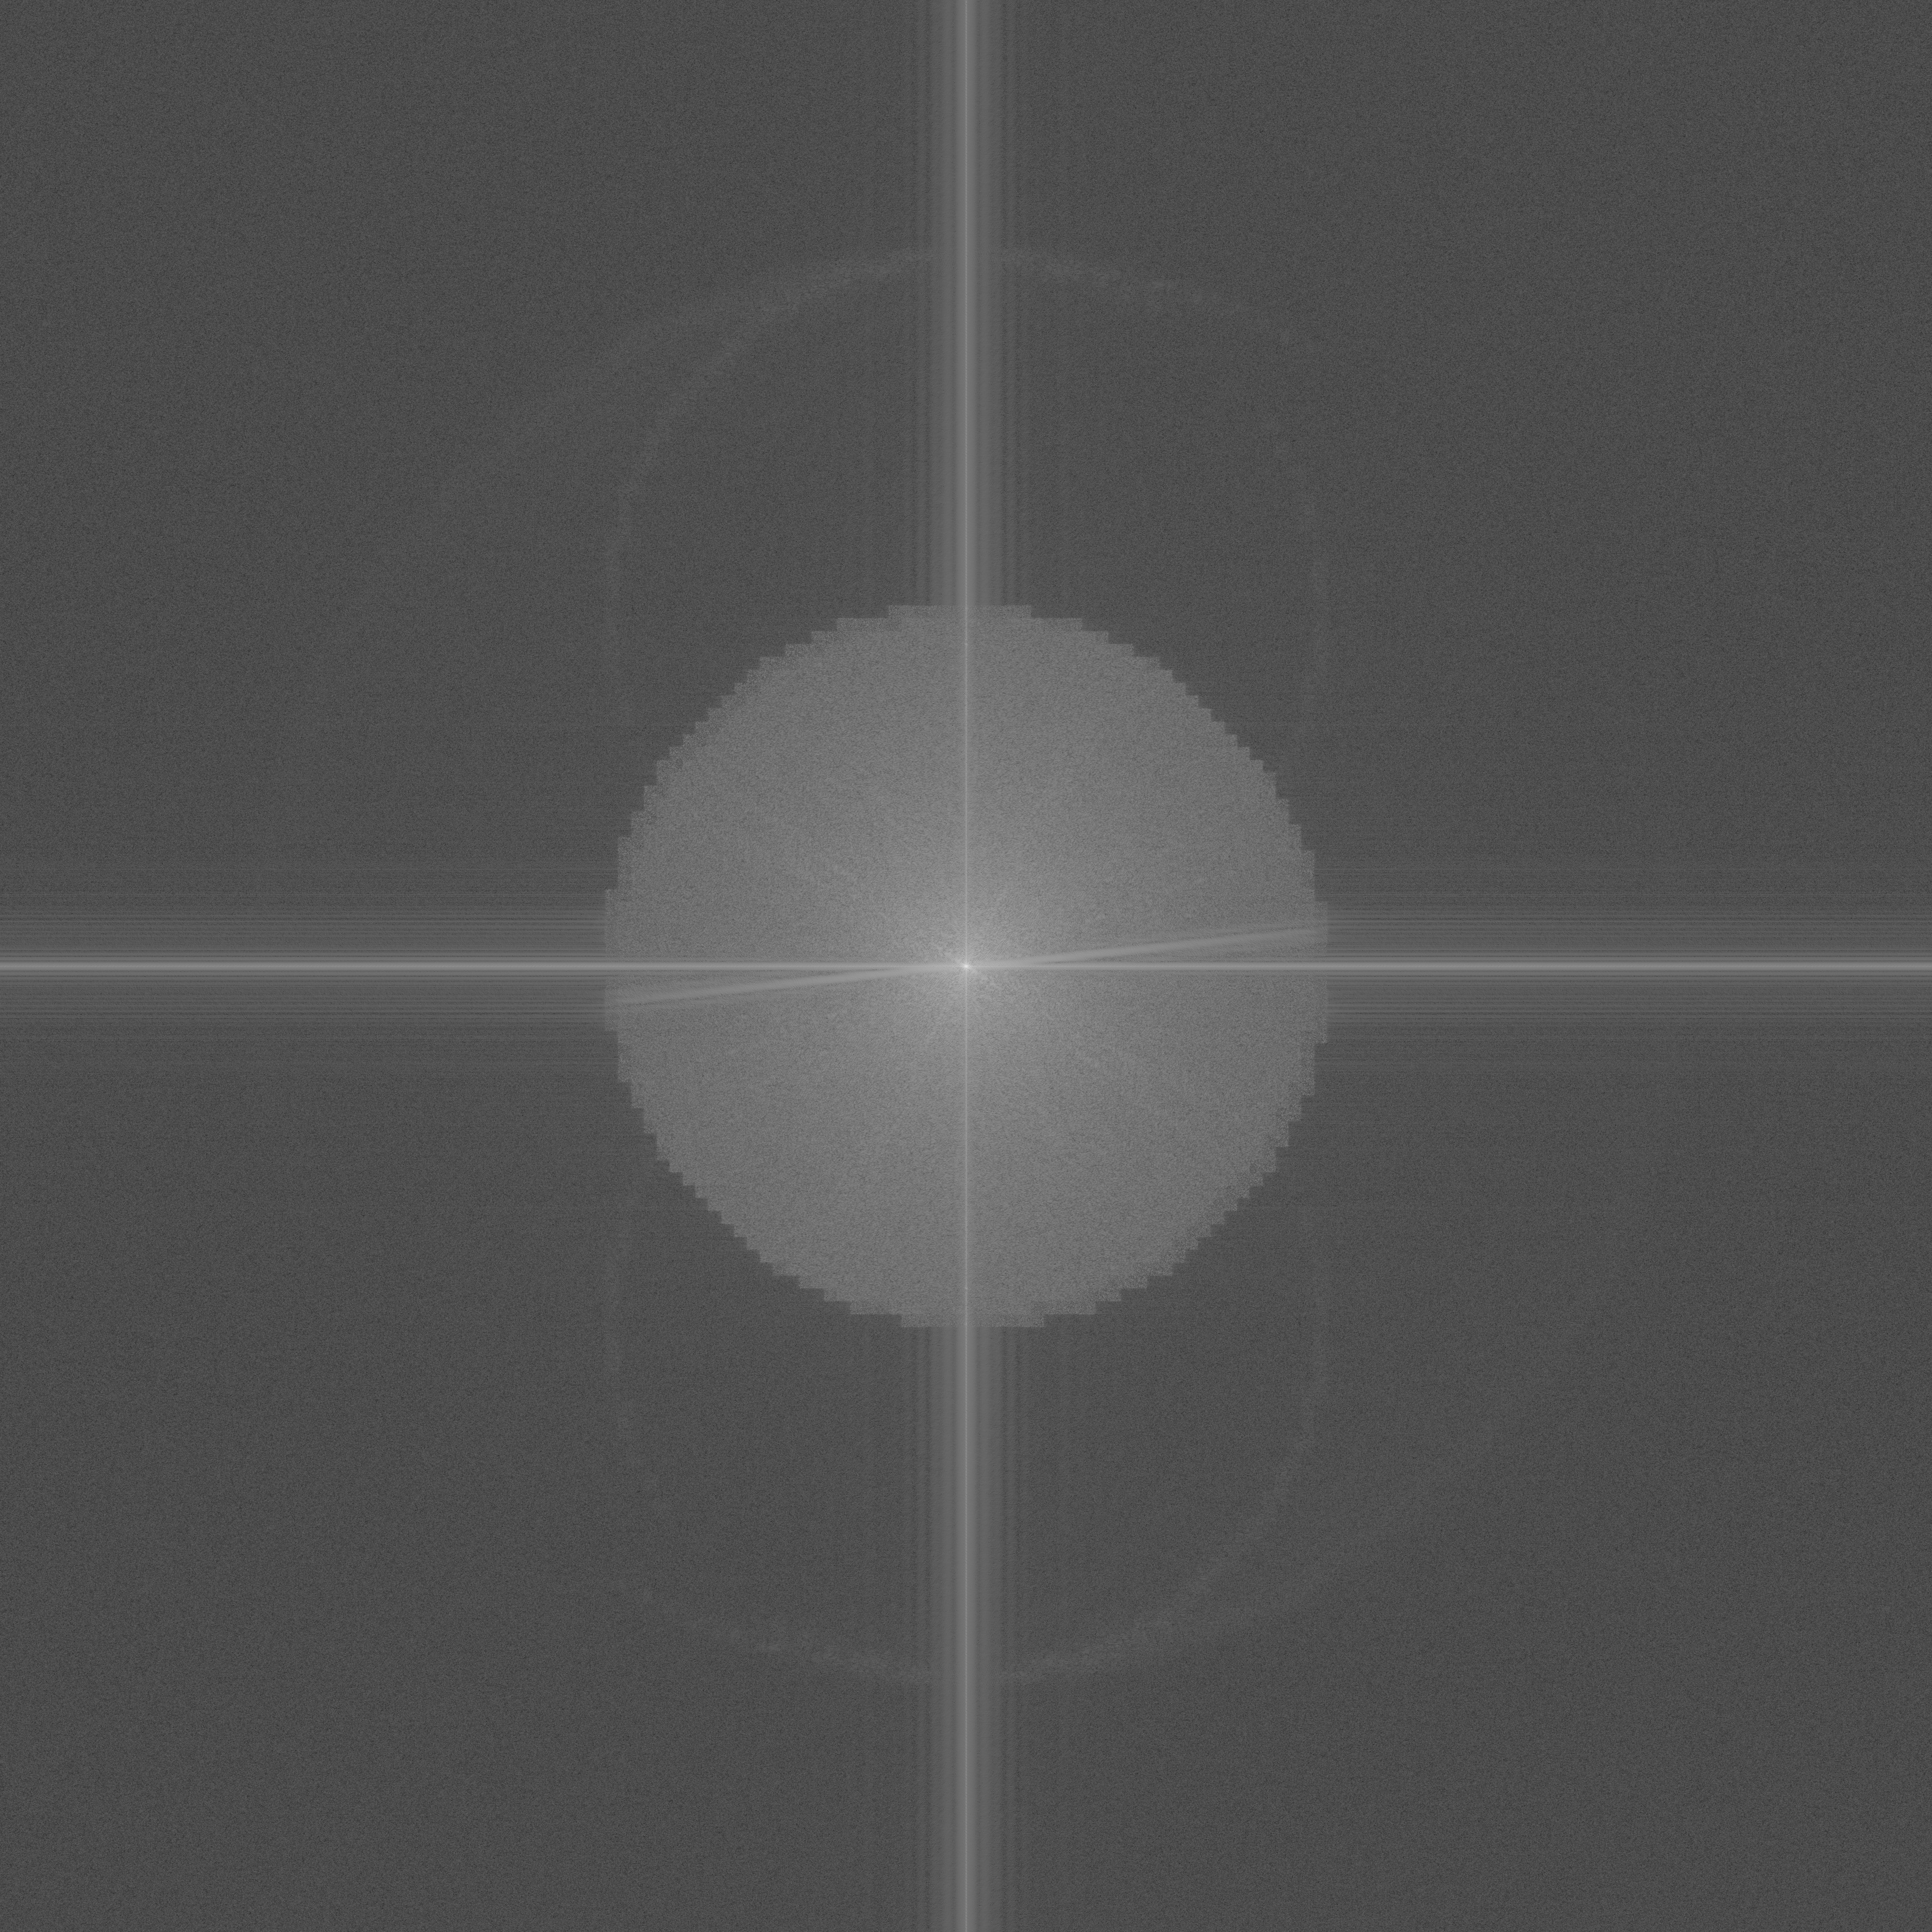
\includegraphics[height=2in]{./immagini_terza_prova/tetta_1/FFTofgriglia_mammo_fft.jpg}
	
\end{subfigure}%
\bigbreak

%%%%%%%%%%%%%%%%%%%%%%%%%%%%%%%%

\begin{subfigure}[b]{0.5\textwidth}
	\centering
	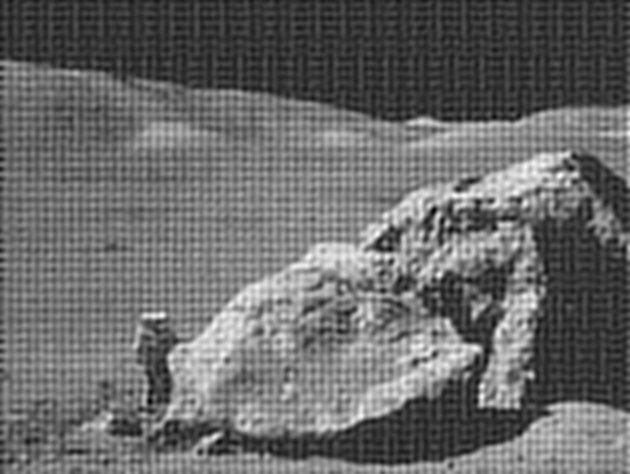
\includegraphics[height=1.7in]{./immagini_terza_prova/moon_1/moonlanding_fft.jpg}
	
\end{subfigure}%
\begin{subfigure}[b]{0.5\textwidth}
	\centering
	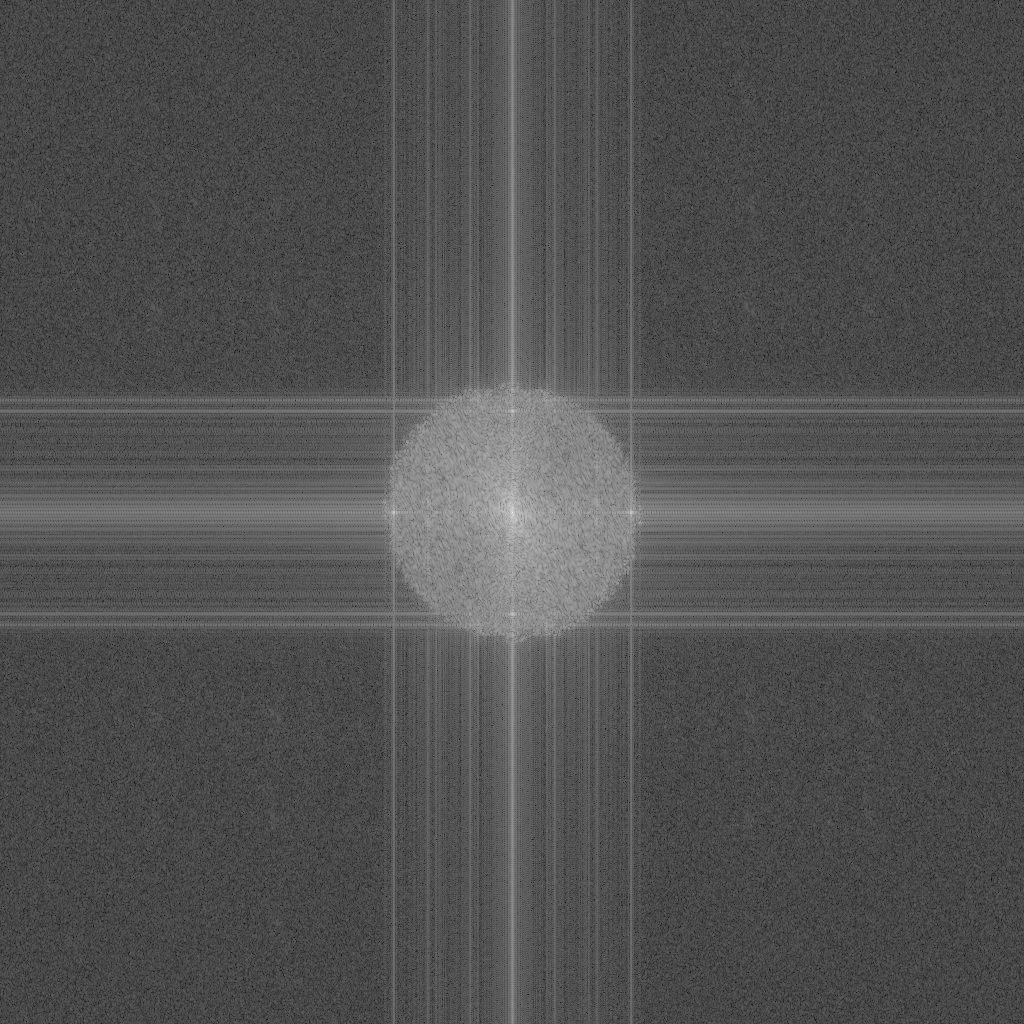
\includegraphics[height=2in]{./immagini_terza_prova/moon_1/FFTofmoonlanding_fft.jpg}
	
\end{subfigure}%

\bigbreak

	\caption{Pictures modified using low-pass frequency filters alongside their respective FFT domain. (From top to bottom) a, b,c}\label{two}
\end{figure}
\clearpage




\section*{Exercise 2}
The second exercise revolved around figure, which is affected by noise created during the acquisition process and contains varios line patterns at different frequencies, measured in $lp/ mm$. Analog to what we did in Exercise 1, we were asked to reduce the noise through operations performed both in the spatial and frequency domains. In this case we were asked to evaluate the effect of the operations by calculating:
\begin{itemize}
\item SNR on a homogenous region , as defined in Exercise 1
\item Spatial  in terms of Modulation transfer functio (MTF) which is defined as:
\begin{equation}
MTF=\frac{M_{out}}{M_{in}}=\frac{Modulation\ in\ recorded\ image}{Iput\ modulation}
\end{equation}
Where $M_{out}$ is given by the contrast in grey levels between the peaks and valleys of averege profiles (the respective histograms, both for the raw and filtered image can be found in Figure 5) of the various line patterns, and $M_{in}$ is assumed t be equal to 40 gray levels in all cases.We decided to perform this operation for both the $2.5\ lp/mm$ and the 
$6.3\ lp/mm$
\end{itemize}
We decided to apply to the image a gaussian filter in the spatial domain 
and a low pass filter, the effect of which can be found in Figure. The SNR and MTF values are instead tabled in Table 2.
\\
\begin{table}[h]
	\begin {center}
	\begin{tabular}{| l | l | l | l | }
		\hline
		Pattern & Operation & SNR & MTF \\ \hline
		$2.5\ lp/mm$& raw & 6.78 & 11.12 \\ \hline
		& gaussian filter & 3.65 & 23.33 \\ \hline 
		& low-pass filter & 3.65 & 24.60 \\ \hline 
		$6.3\ lp/mm$& raw & 6.78 & 11.12 \\ \hline
		& gaussian filter & 3.65 & 23.33 \\ \hline 
		& low-pass filter & 3.65 & 24.60 \\ \hline 
	\end{tabular}
	\caption{da riempire}
\end{center}
\end{table}
\clearpage
\begin{figure}[h]
	\centering
	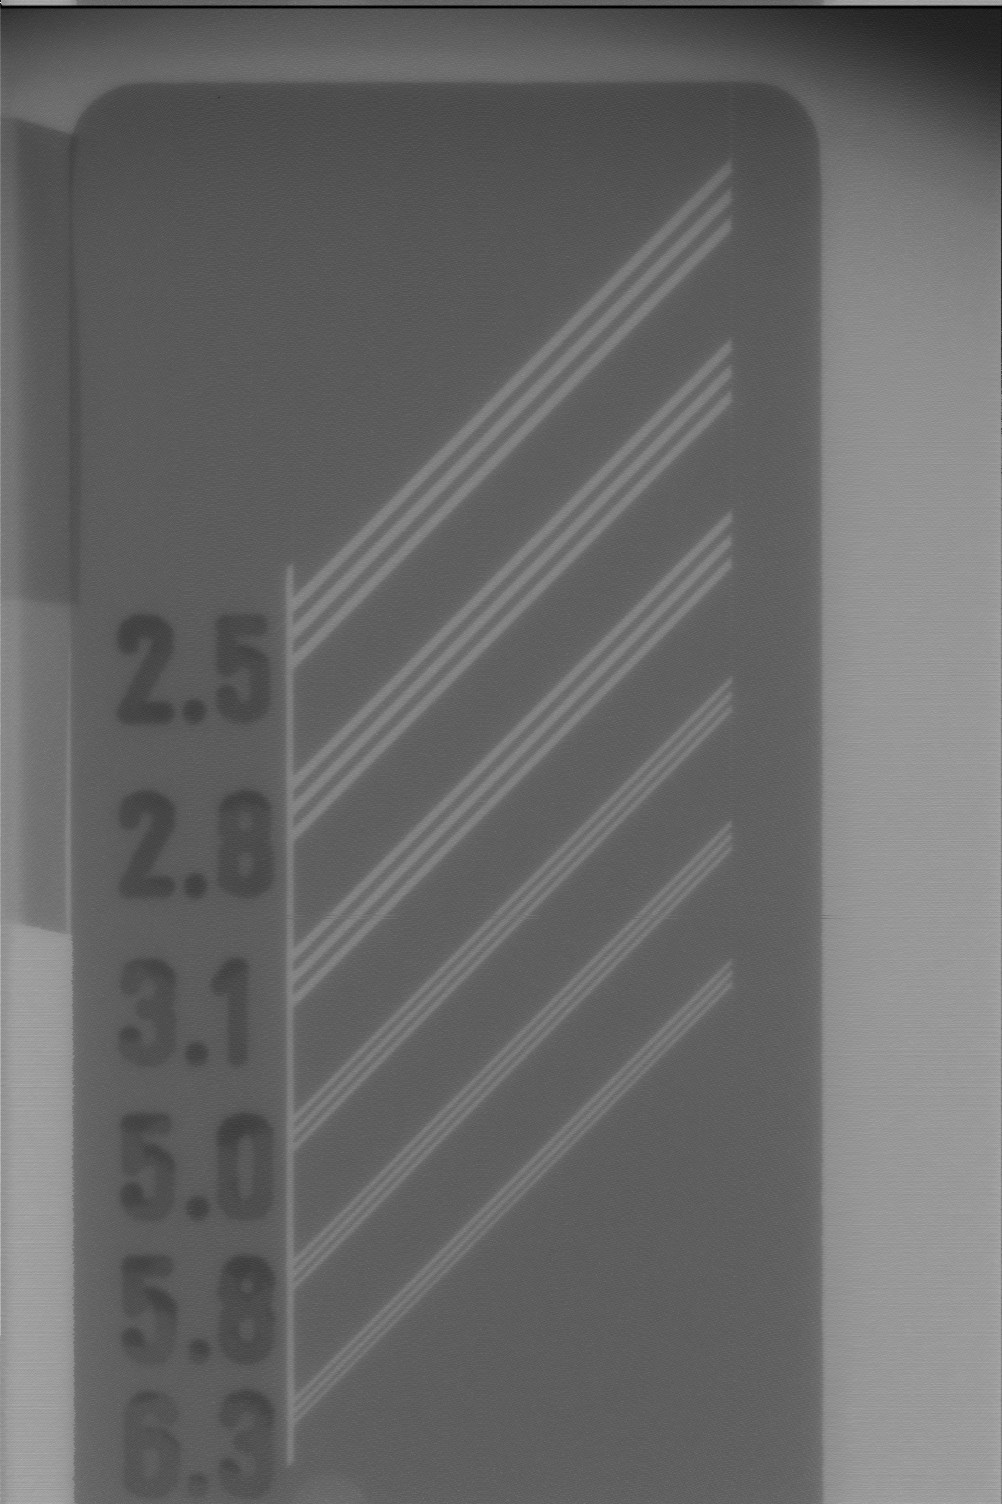
\includegraphics[width=.33\textwidth]{./immagini_terza_prova/ex2/raw0.jpg}
	\bigbreak
	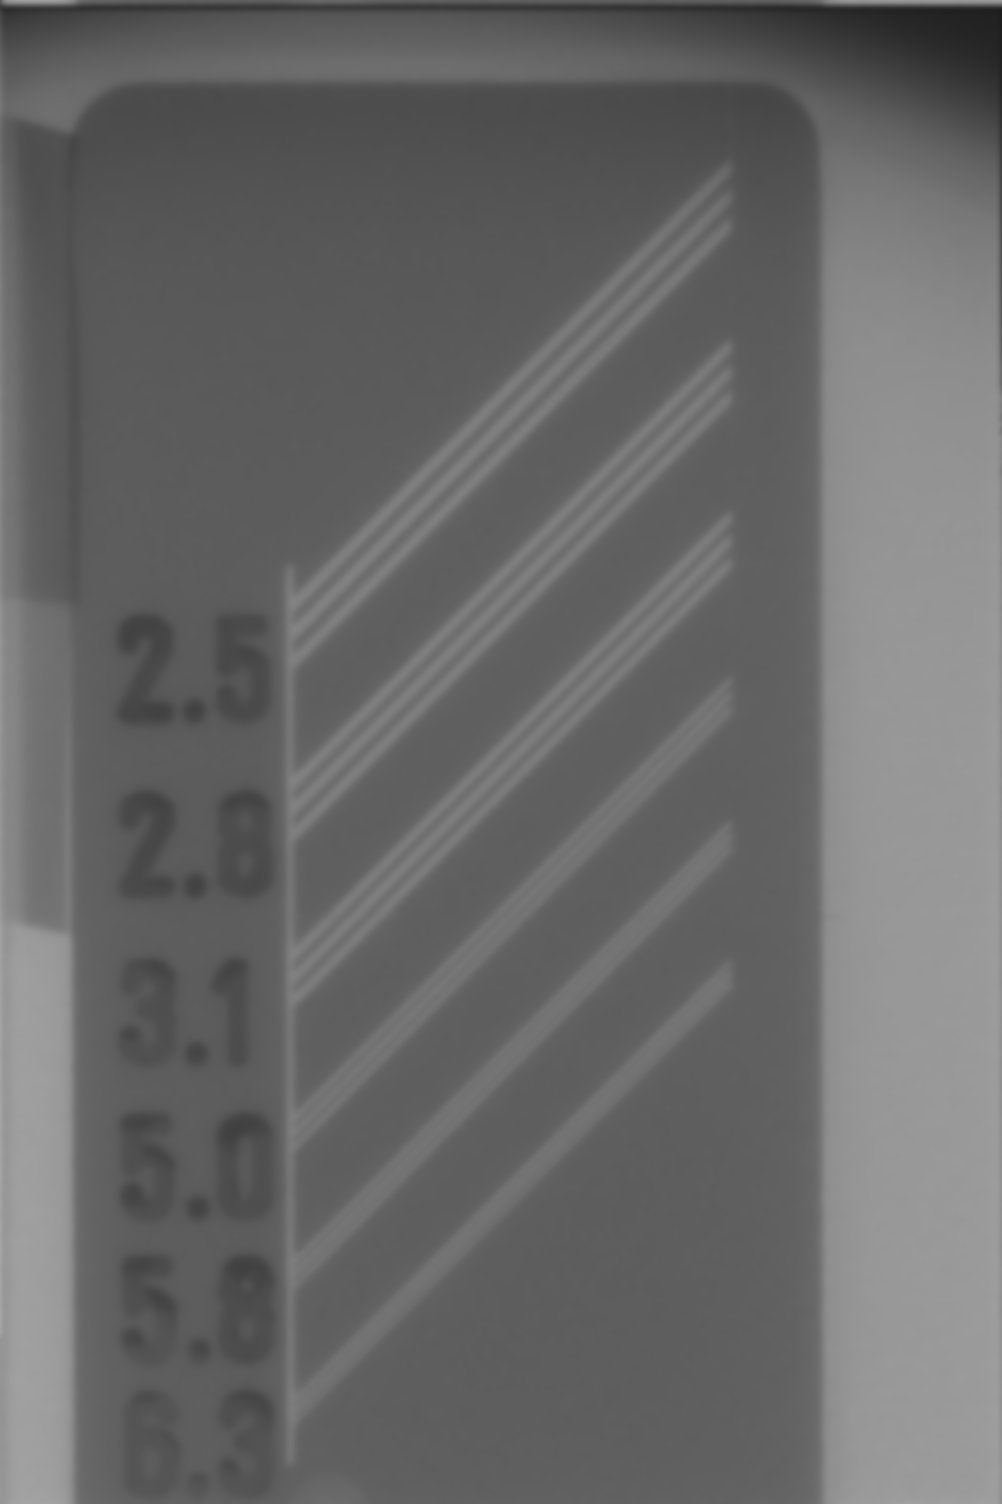
\includegraphics[width=.33\textwidth]{./immagini_terza_prova/ex2/gaussian.jpg}
	\bigbreak
	\begin{subfigure}[b]{0.5\textwidth}
		\centering
		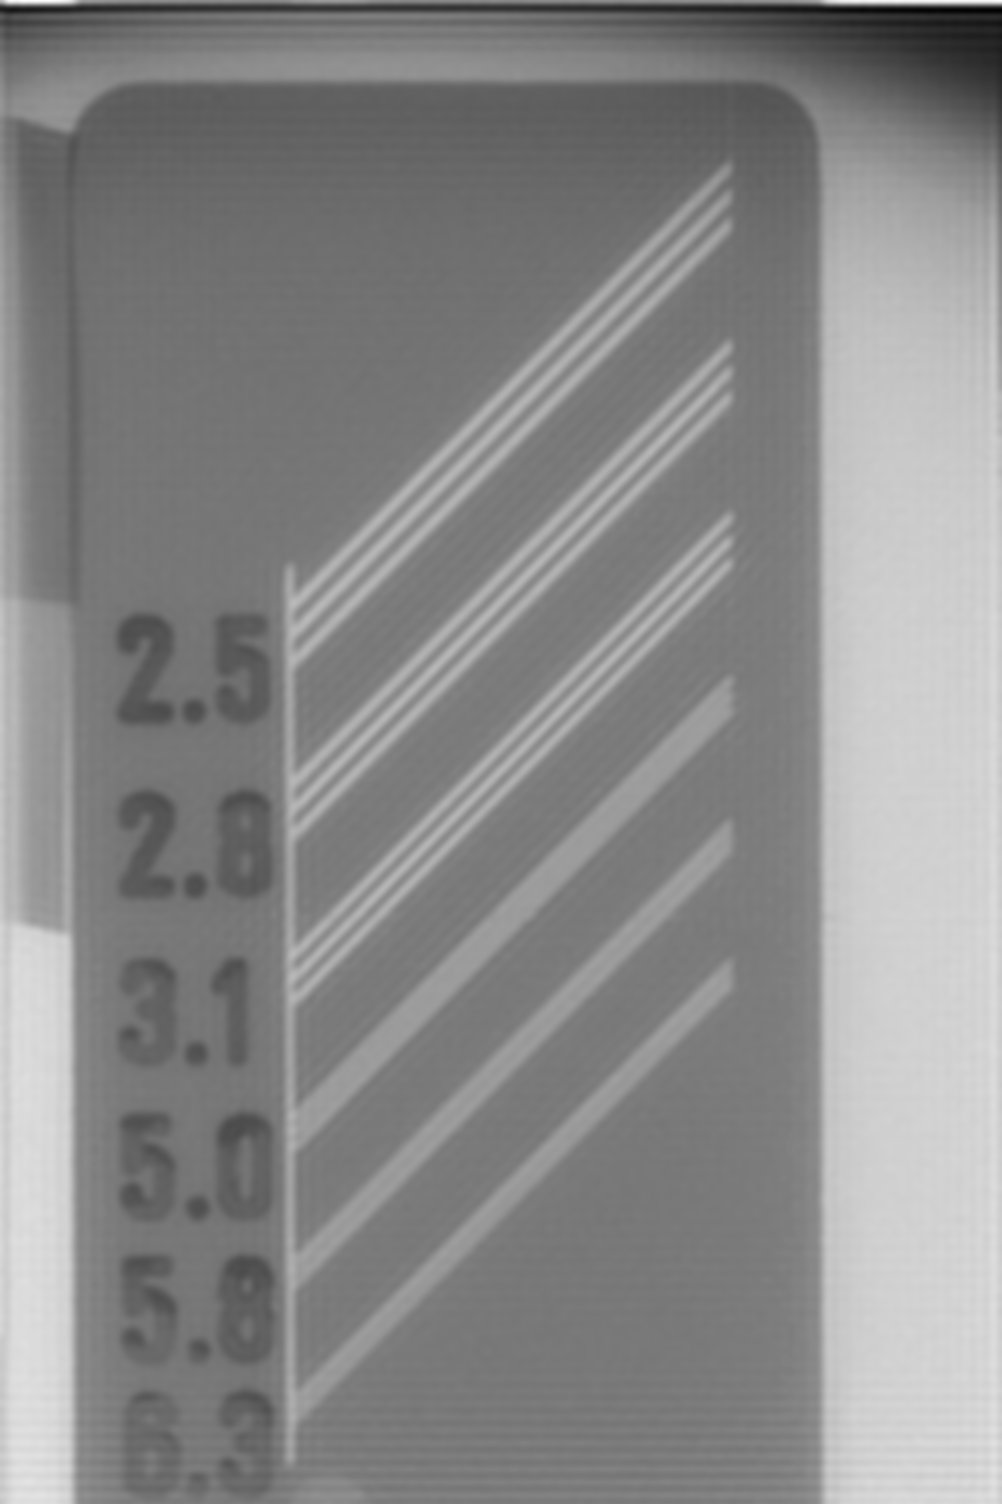
\includegraphics[height=2in]{./immagini_terza_prova/ex2/raw0_fft.jpg}
		
	\end{subfigure}%
	\begin{subfigure}[b]{0.5\textwidth}
		\centering
		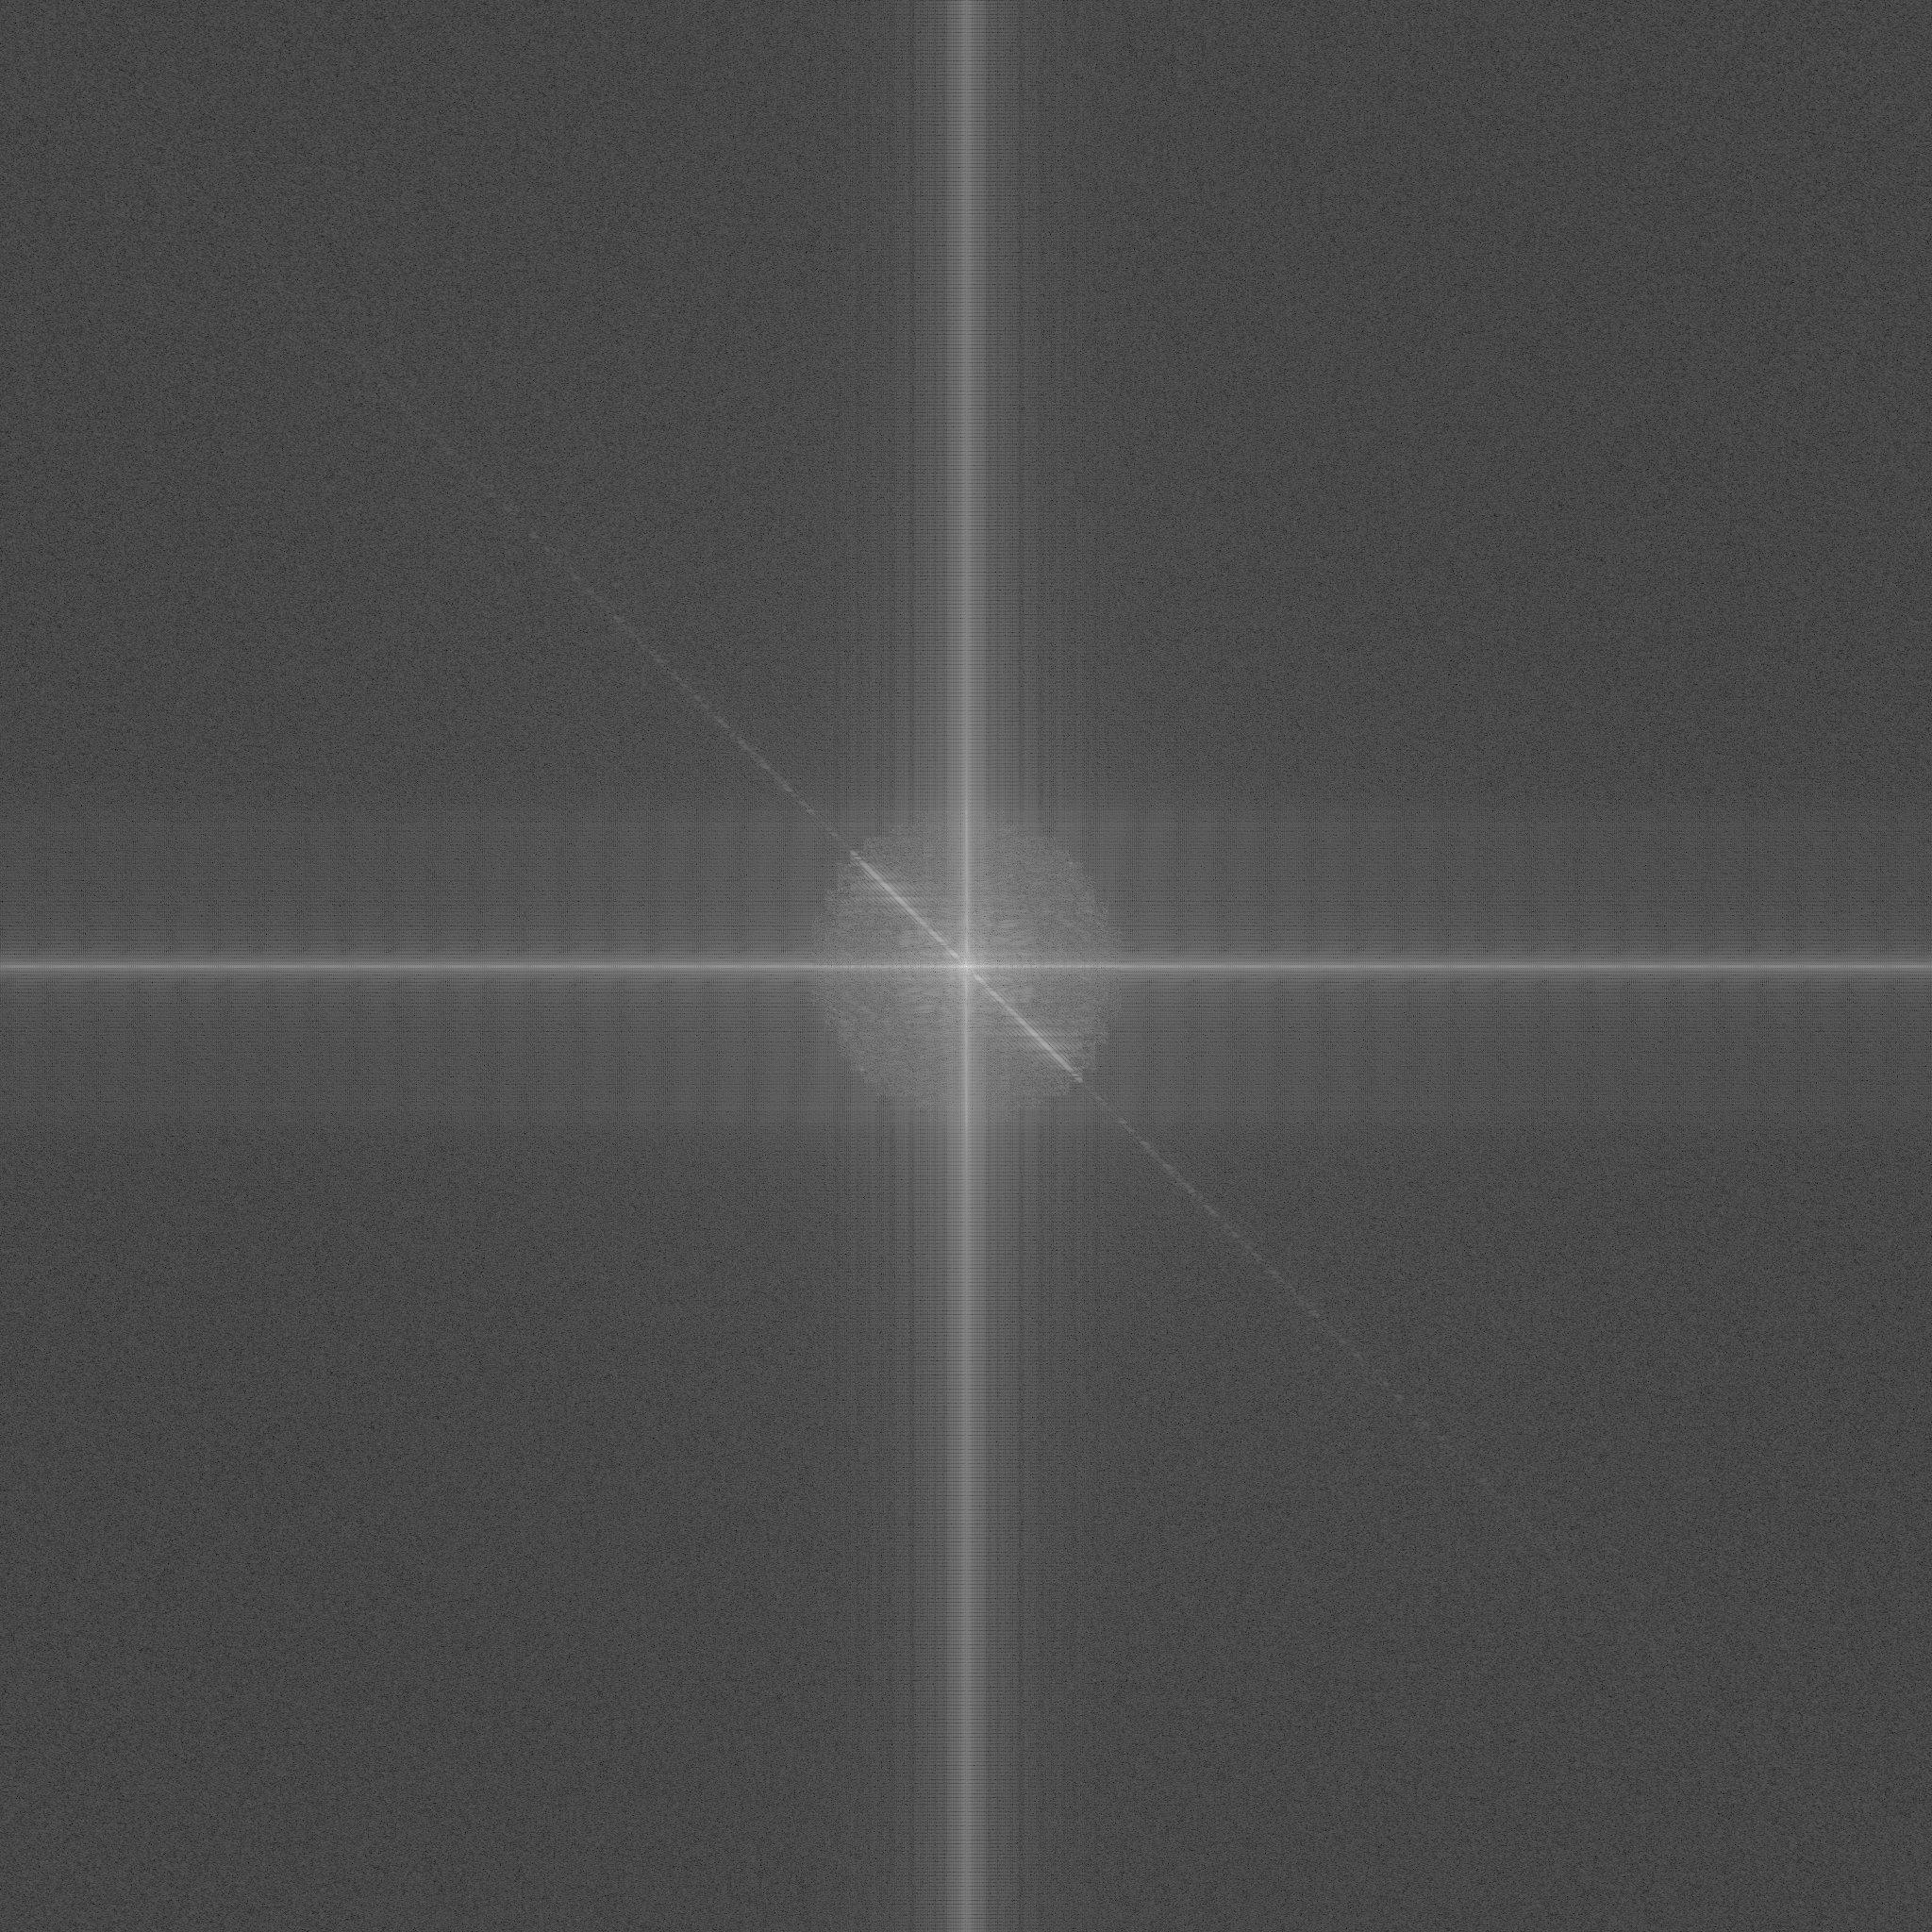
\includegraphics[height=2in]{./immagini_terza_prova/ex2/FFTofraw0_fft.jpg}
		
	\end{subfigure}%
	
	\bigbreak
	
	\caption{ (From top to bottom) a: Raw line patterns picture; b: Picture modified with gaussian filter  ; c: Picture modified with low-pass filter alongside its frequency spectrum}\label{two}
\end{figure}

\begin{figure}[h]
	\centering
	\begin{subfigure}[b]{0.5\textwidth}
		\centering
		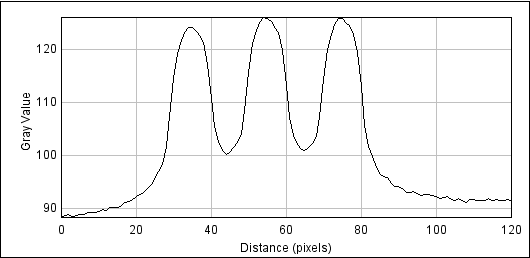
\includegraphics[height=1.15in]{./immagini_terza_prova/ex2/25_profile_histo_raw.PNG}
		
	\end{subfigure}%
	\begin{subfigure}[b]{0.5\textwidth}
		\centering
		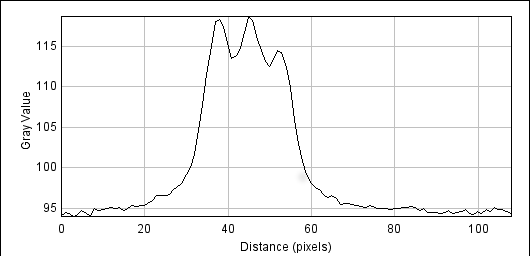
\includegraphics[height=1.15in]{./immagini_terza_prova/ex2/62_prof_histo_raw.PNG}
		
	\end{subfigure}%
	\bigbreak
	%%%%%%%%%%%%%%%%%%%%%%%%%%%%%%%%%%%%%
	\begin{subfigure}[b]{0.5\textwidth}
		\centering
		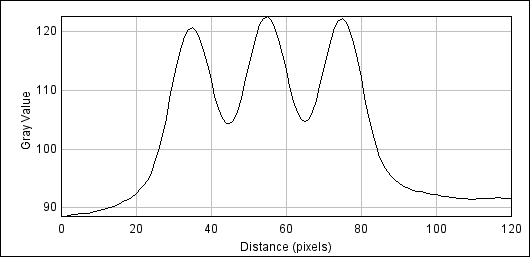
\includegraphics[height=1.15in]{./immagini_terza_prova/ex2/25_prof_histo_gaussian.PNG}
		
	\end{subfigure}%
	\begin{subfigure}[b]{0.5\textwidth}
		\centering
		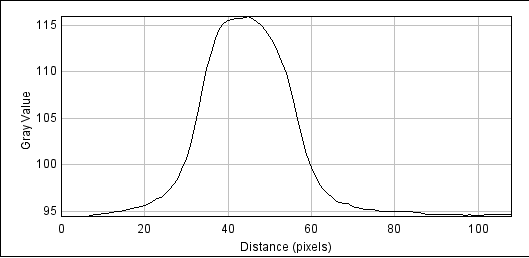
\includegraphics[height=1.15in]{./immagini_terza_prova/ex2/62_prof_histo_gaussian.png}
		
	\end{subfigure}%
	\bigbreak
	%%%%%%%%%%%%%%%%%%%%%%%%%%%%%%%%%%%%%
		\begin{subfigure}[b]{0.5\textwidth}
			\centering
			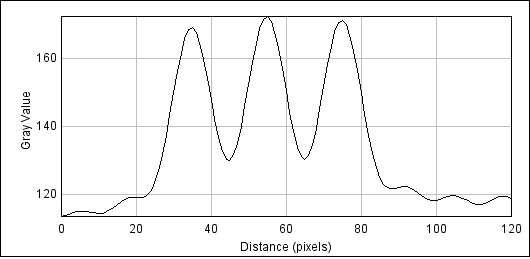
\includegraphics[height=1.15in]{./immagini_terza_prova/ex2/25_prof_histo_fft.PNG}
			
		\end{subfigure}%
		\begin{subfigure}[b]{0.5\textwidth}
			\centering
			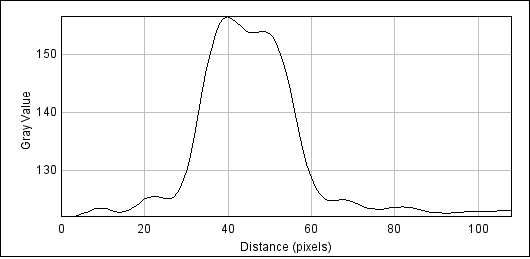
\includegraphics[height=1.15in]{./immagini_terza_prova/ex2/62_prof_histo_fft.PNG}
			
		\end{subfigure}%
		\bigbreak

	
	\caption{(From top to bottom) a: Averaged profile histogram of the raw picture for the $2.5\ lp/mm$ pattern (left) and $6.3\ lp/mm$ pattern (right); b: Averaged profile histogram of the gaussian filtered picture for the $2.5\ lp/mm$ pattern (left) and $6.3\ lp/mm$ pattern (right)  ; c: Averaged profile histogram of the low-pass filtered picture for the $2.5\ lp/mm$ pattern (left) and $6.3\ lp/mm$ pattern (right)}\label{two}
\end{figure}
\clearpage
\section*{Exersize 3}
For Exercise 3 we were asked to perform a flat-field correction on the mammographic image in Figure,. This operation can be performed by subtracting pixel by pixel a flat-field image from our raw image and multiplying by a normalization constant:
\begin{equation}
IC=(\frac{IR}{IF})* M
\end{equation}
Where IC is the corrected image (Figure 6c), IR is the raw image (Figure 6a), IF is the flat-field image (Figure6b)and M is the normalization constant, which in this case is assumed to be equal to 100.
We were then asked to evaluate the image quality using:
\begin{itemize}
	\item Profile and SNR on an extended area outside the phantom (as described in Exercise 1)
	\item Contrast to noise ratio (CNR) evaluated on the circular inserts within the phantom, by applying the formula:
	\begin{equation}
	CNR=\frac{I_{detail}-I_{background}}{\sigma_{background}}
	\end{equation}
	Where $I_{detail}$ and $I_{background}$ the averege grey level of the detail and a homogenous area of the phantom respectively, and $\sigma_{background}$ is the gray level standard deviation for the same region, which can be interpreted as its noise. We calculated this parameter for two of the the details in the picture.
\end{itemize}
The results of these operations can are tabled in Table 3. 

\begin{table}[h]
	\begin {center}
	\begin{tabular}{| l | l | l | l | l |}
		\hline
		 Operation & $\sigma_{profile}$ & SNR & CNR(1) & CNR(2)\\ \hline
		Raw& raw & 6.78 & 11.12  &\\ \hline
		 Flat-field& gaussian filter & 3.65 & 23.33 &\\ \hline 
		
	\end{tabular}
	\caption{da riempire}
\end{center}
\end{table}
\clearpage

\begin{figure}[h]
	\centering
	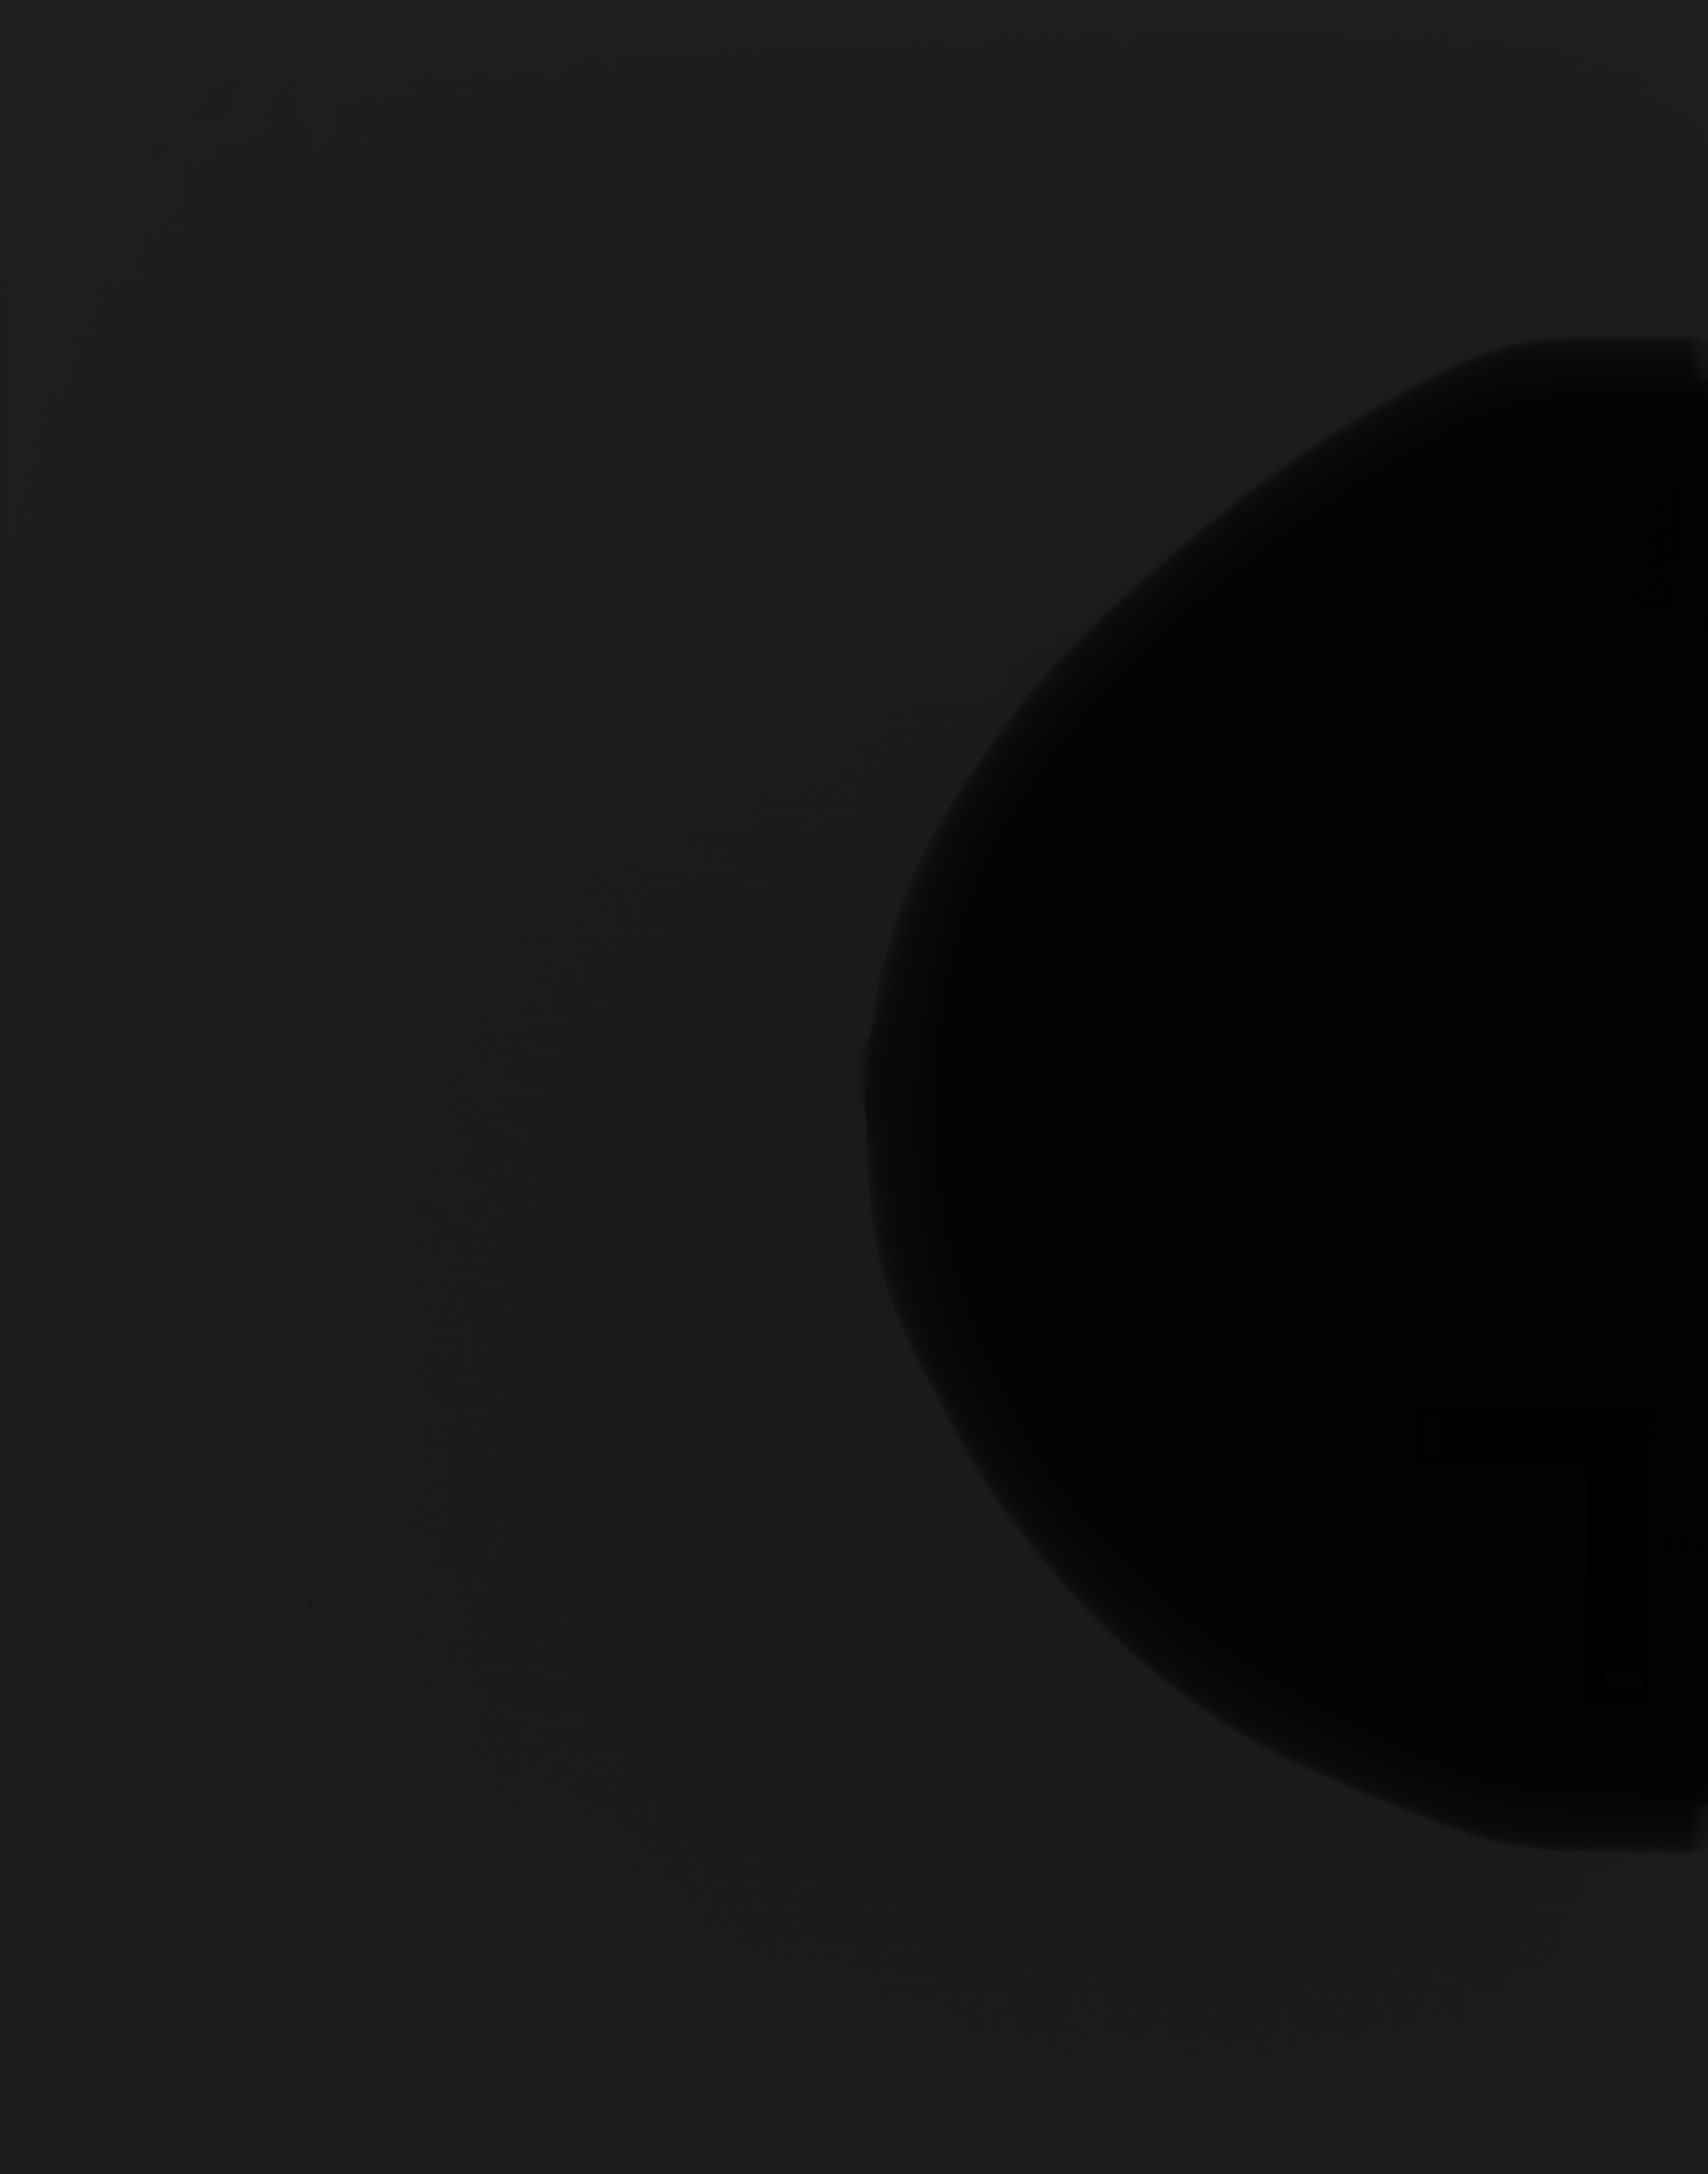
\includegraphics[width=.33\textwidth]{./immagini_terza_prova/ex3/cirs.jpg}
	\bigbreak
	
\includegraphics[width=.33\textwidth]{./immagini_terza_prova/ex3/flat-field.jpg}
	\bigbreak
	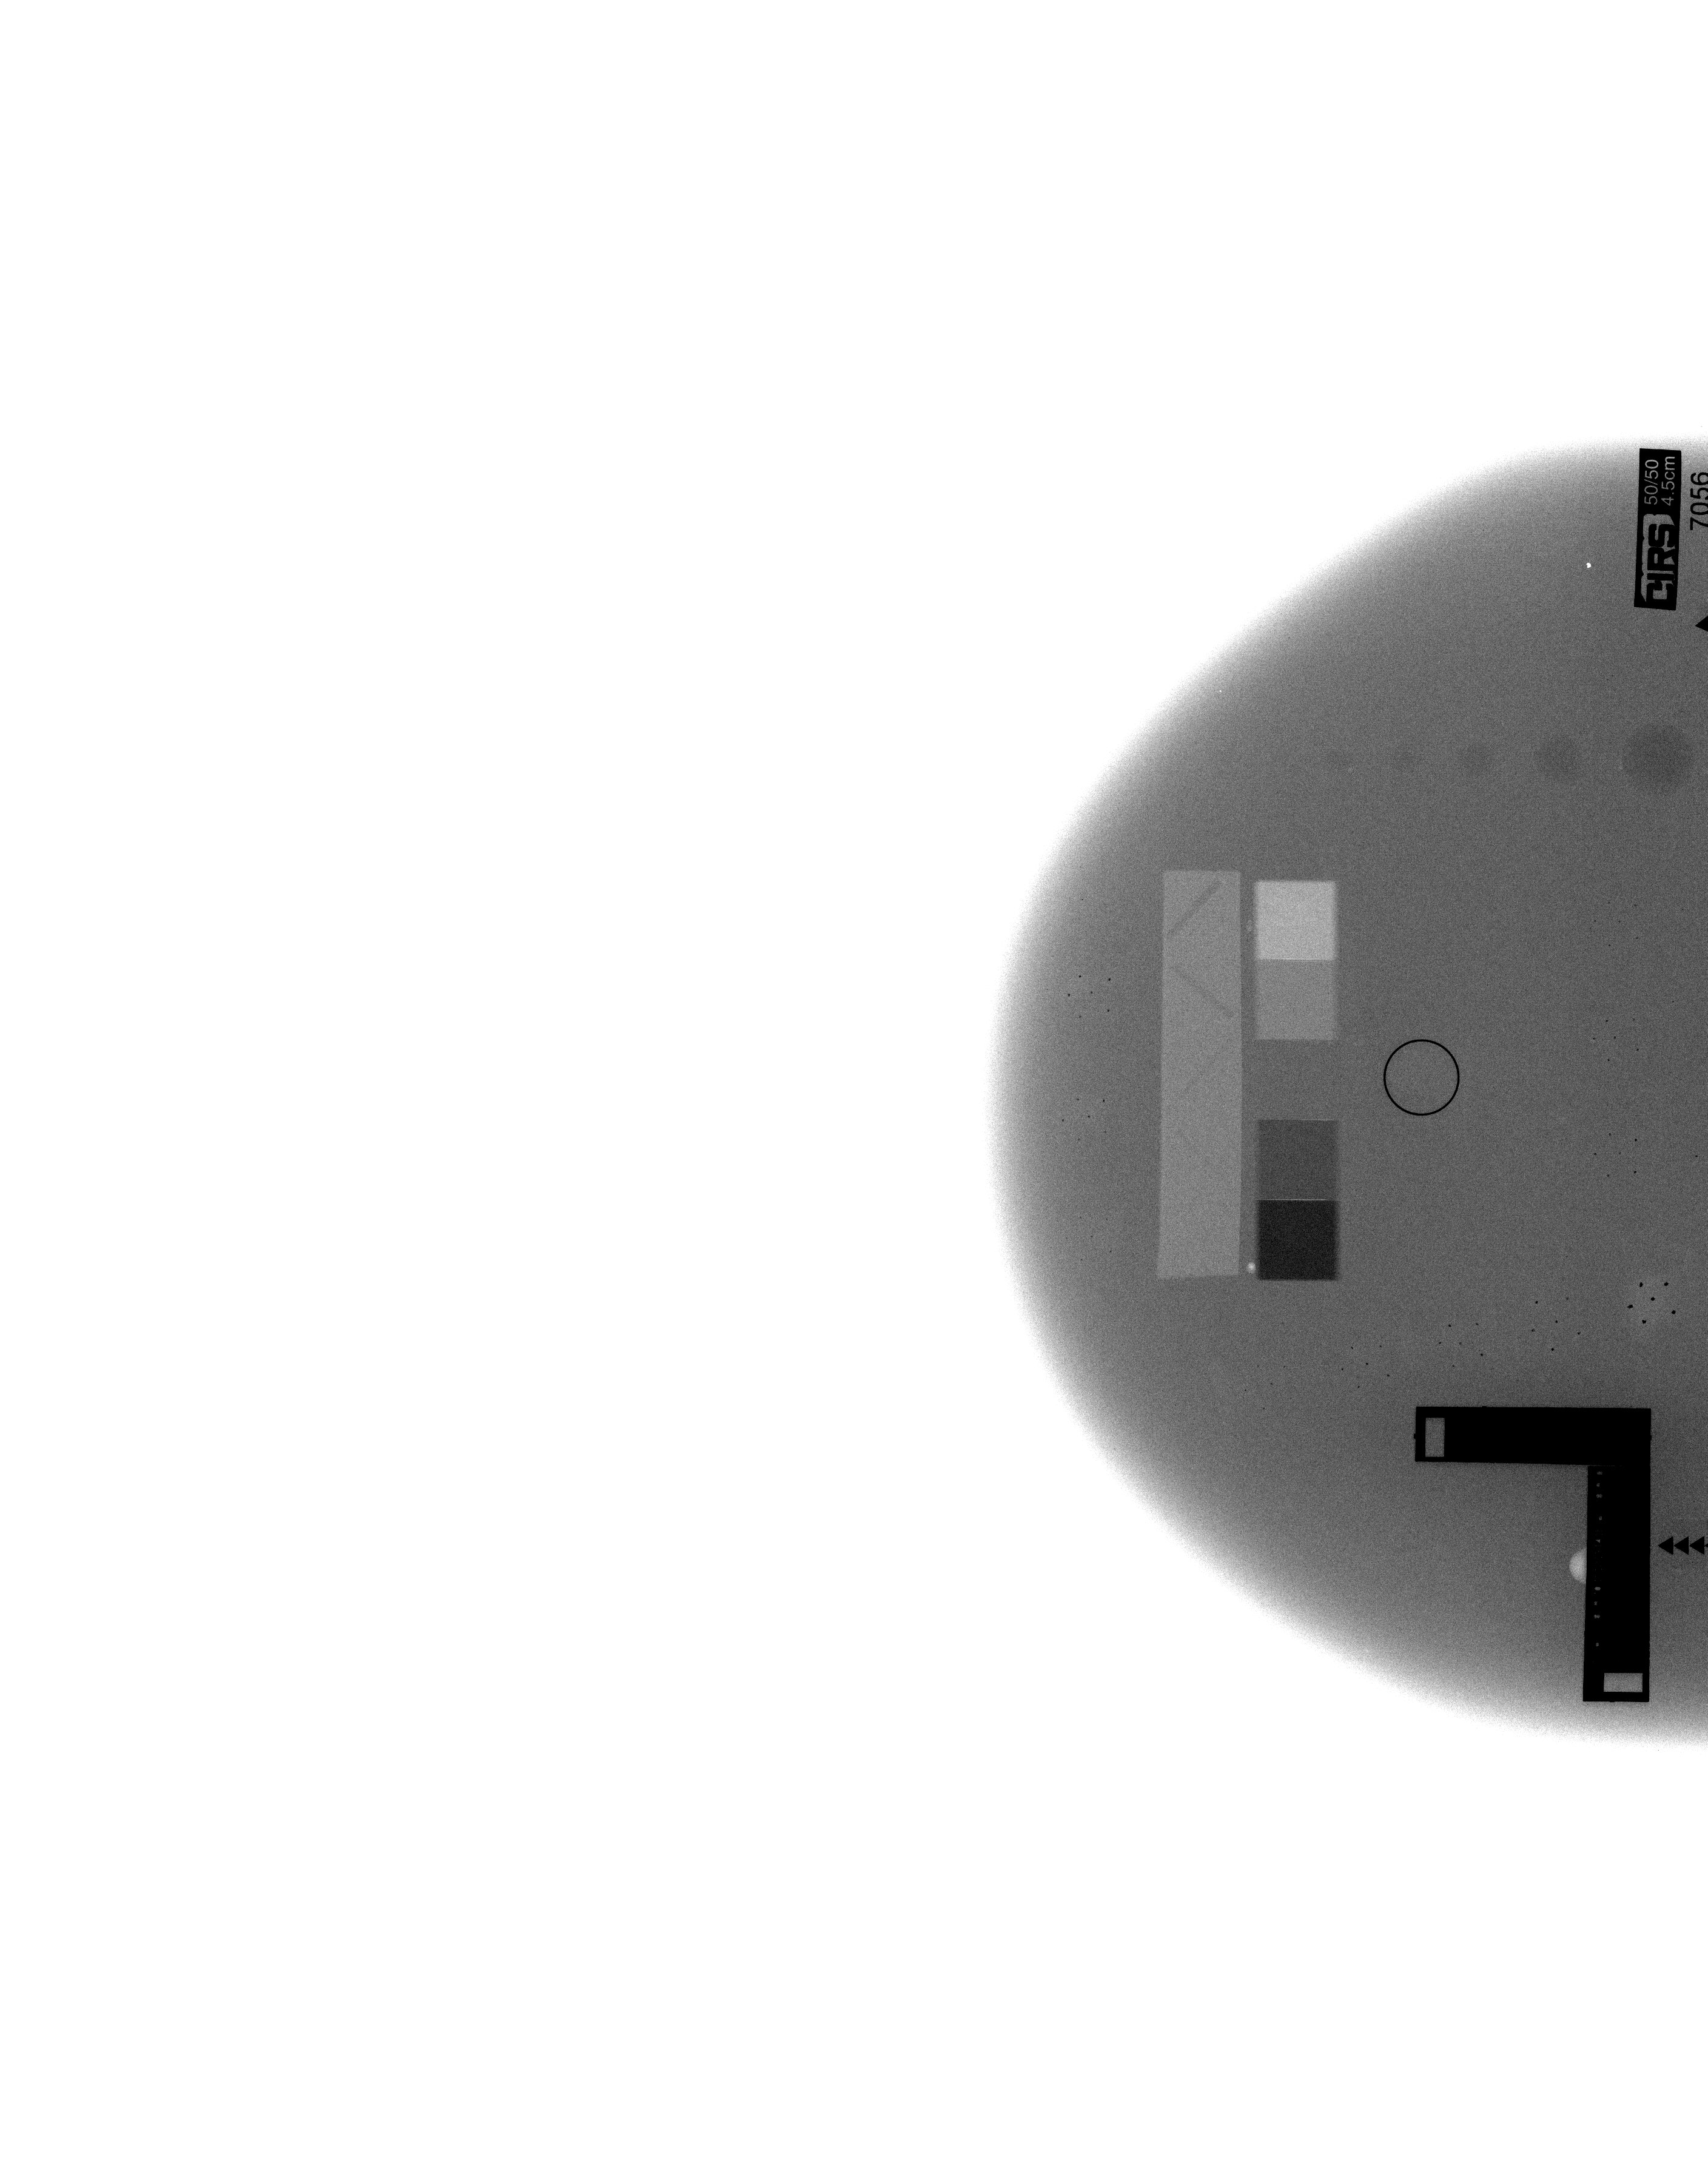
\includegraphics[width=.33\textwidth]{./immagini_terza_prova/ex3/Resultofcirs.jpg}
	\bigbreak
	
	\caption{ (From top to bottom) a: Raw mammographic picture with circular details within the phantom; b: Flat-field image ; c: Flat-field corrected image}\label{two}
\end{figure}
\clearpage
\section*{Exercise 4}
For the last session of the experience we were asked to evaluate the performance of the detection system , through a contrast-detail analysis  performed on Figure, which shows a picture (obtained with the detection system itself)of a table containing various circular shapes with different diameters (decreasing from top to bottom) and different levels of contrast with the background (decreasing from right to left). \\
To this end we calculated the CNR on the central detail for all cells relative to the three diameters: 6.3mm, 4.0mm and 2.5mm. these values can be found graphed as a function of the thickness of the details in Figure.

\begin{figure}[h]
	\centering
	\bigbreak
	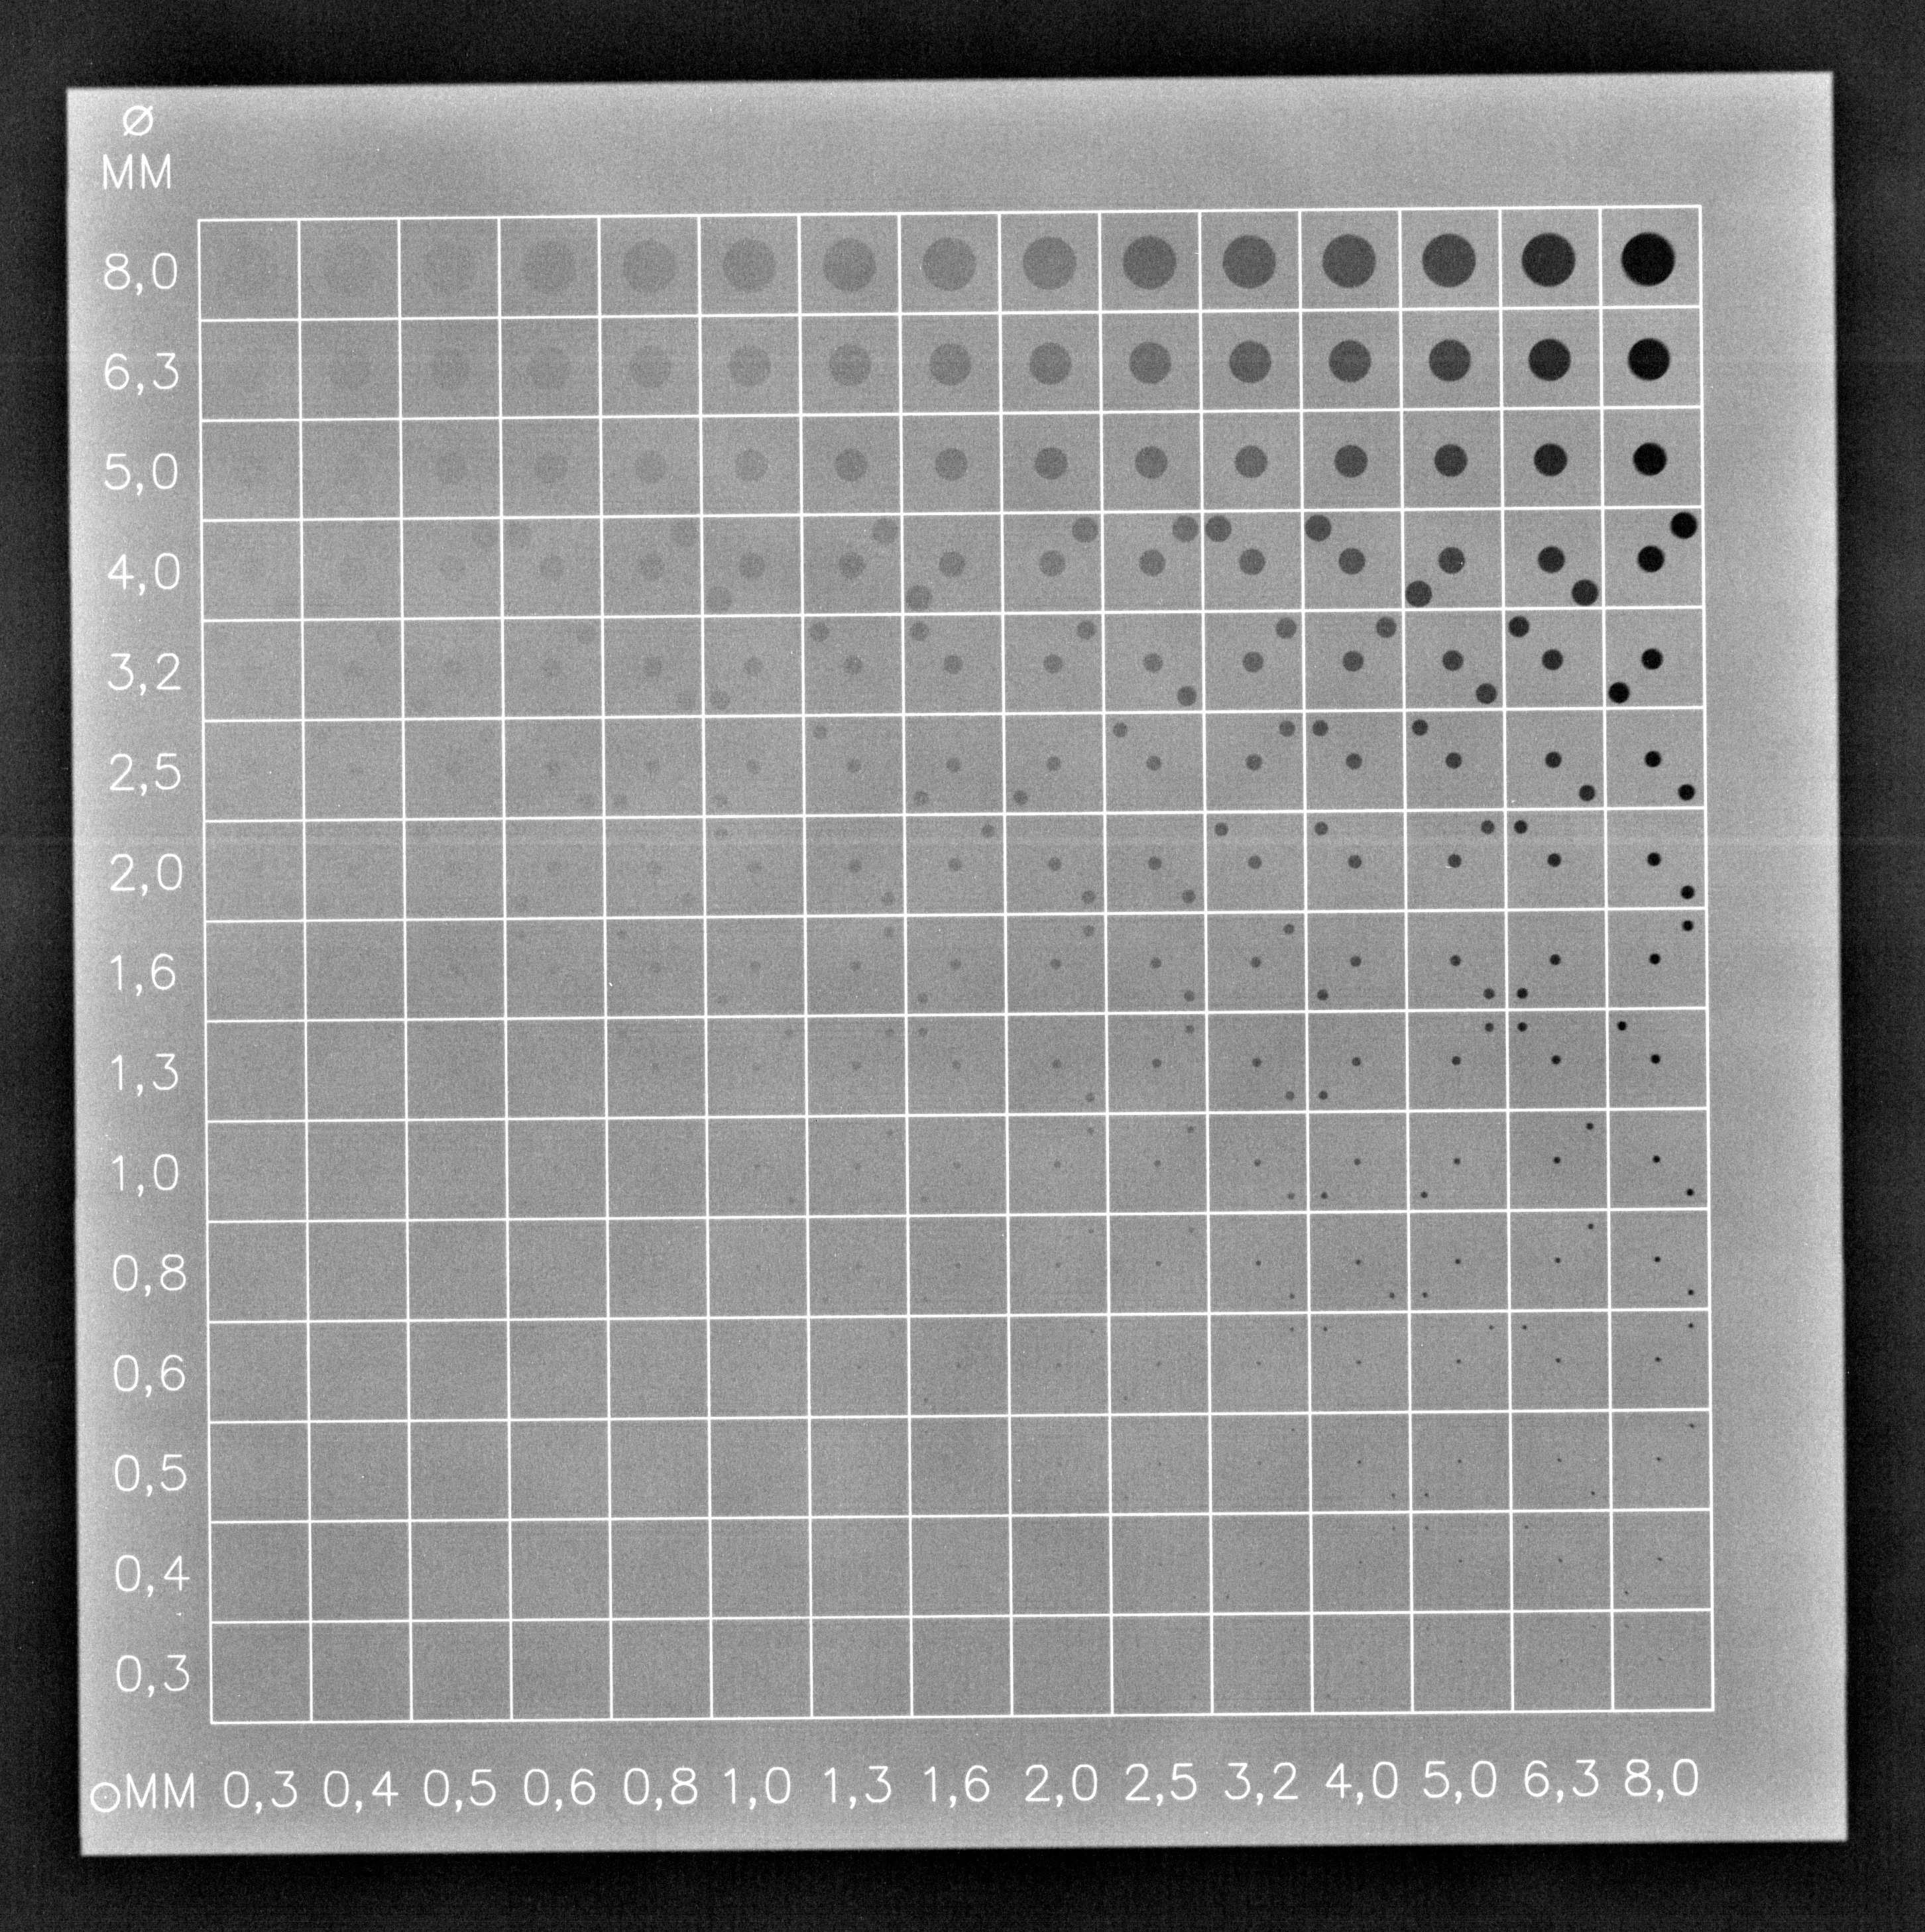
\includegraphics[width=0.8\textwidth]{./immagini_terza_prova/ex4/CDRAD-10_3.jpg}
	\bigbreak
	\caption{Picture of the phantom we used toevaluate the performance of the detection system   }\label{two}
\end{figure}
\clearpage
\begin{figure}[h]
	\centering
	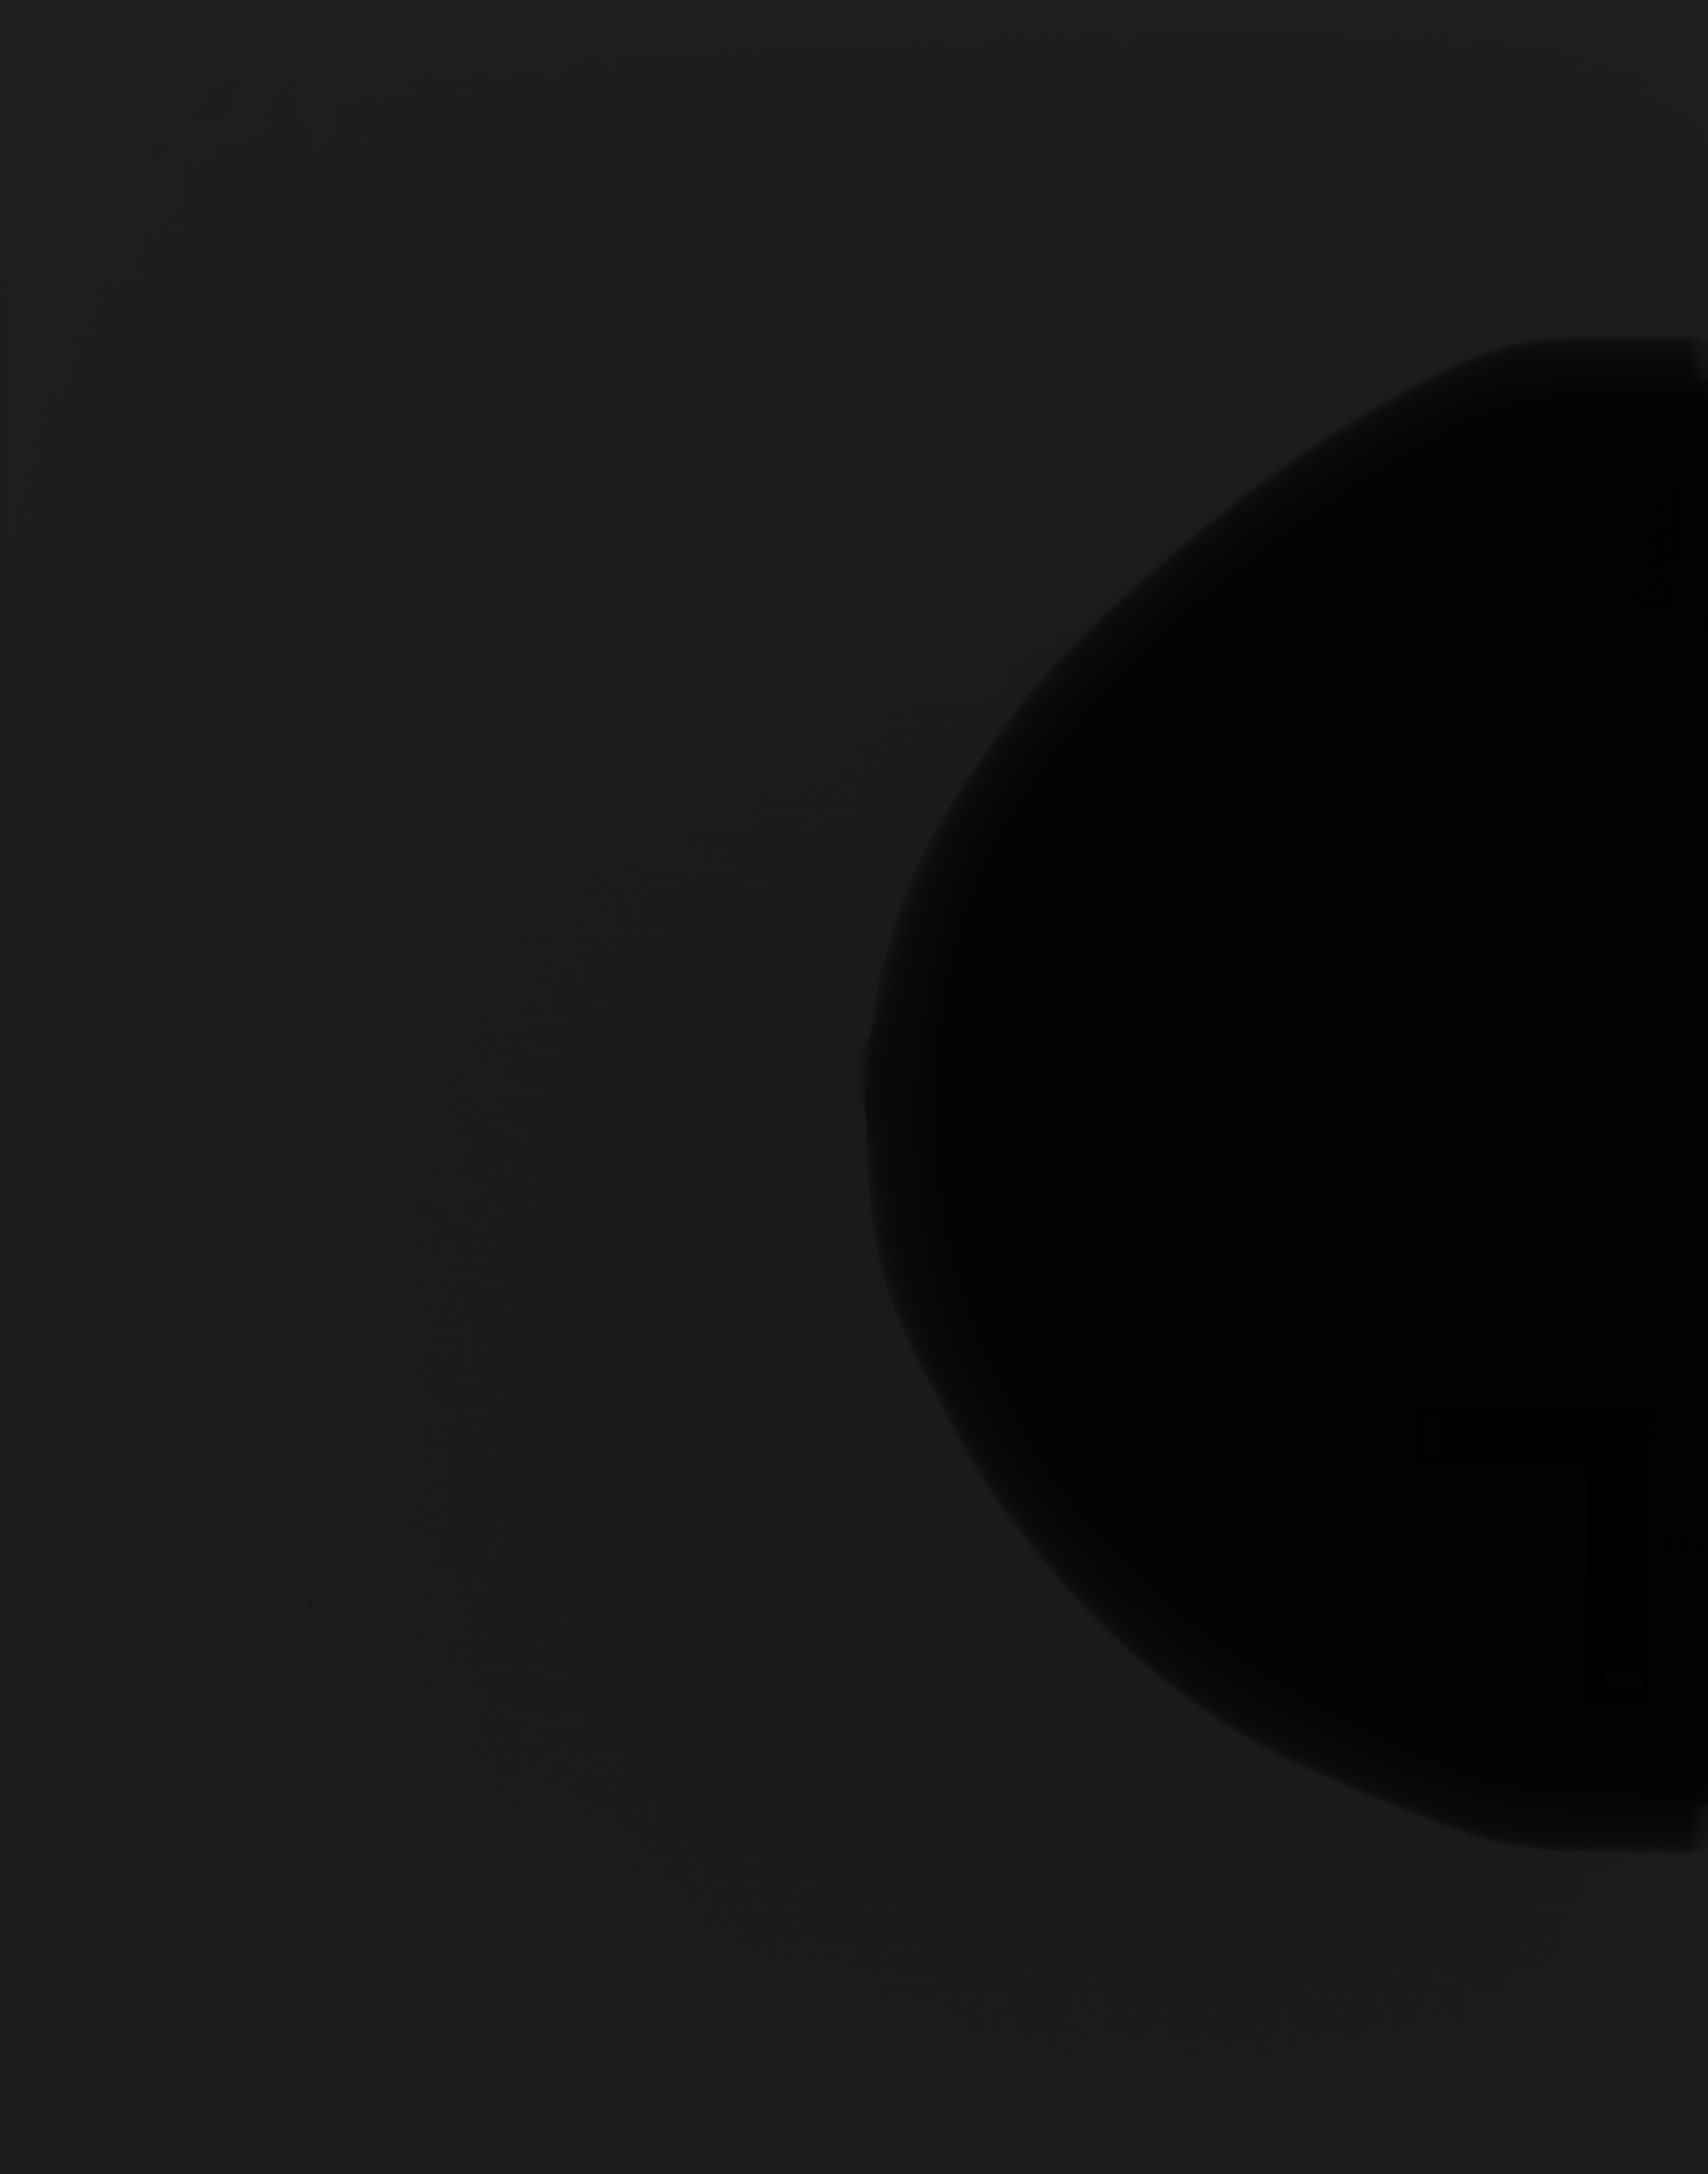
\includegraphics[width=.33\textwidth]{./immagini_terza_prova/ex3/cirs.jpg}
	\bigbreak
	
\includegraphics[width=.33\textwidth]{./immagini_terza_prova/ex3/flat-field.jpg}
	\bigbreak
	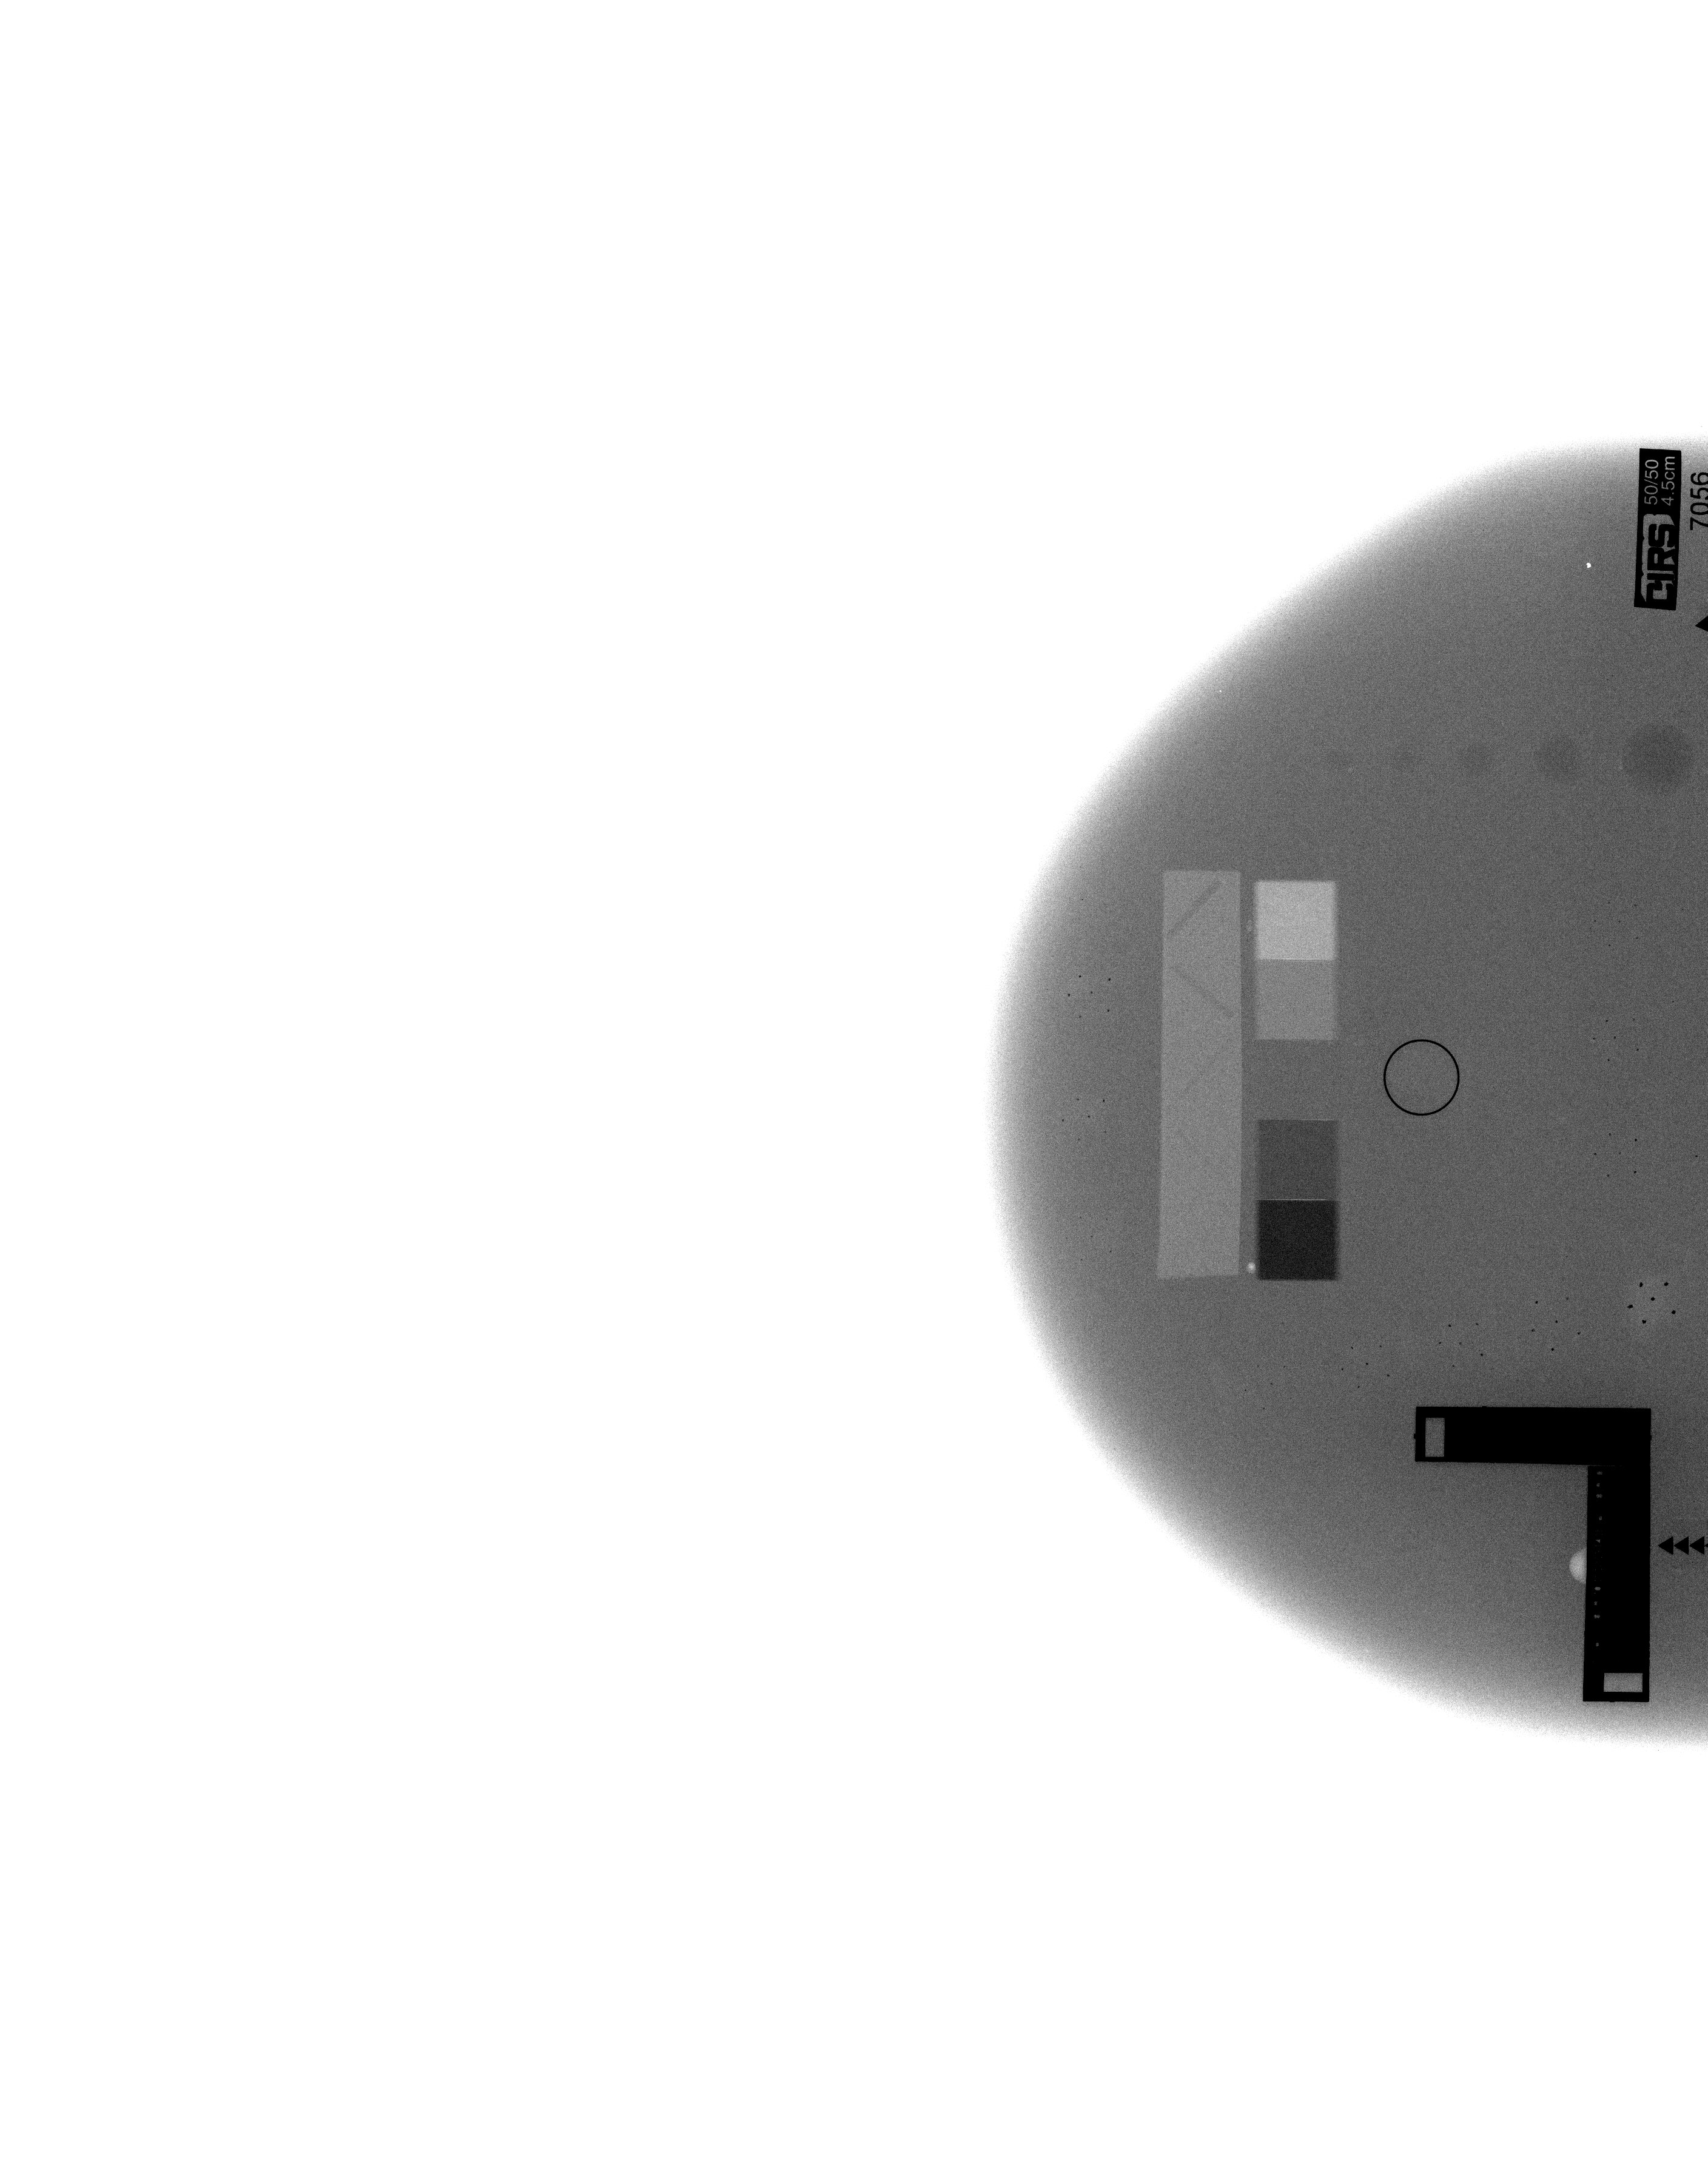
\includegraphics[width=.33\textwidth]{./immagini_terza_prova/ex3/Resultofcirs.jpg}
	\bigbreak
	
	\caption{ Value of CNRas a function of the thickness of the details of diameter: (From top to bottom) a- 6.3 mm b- 4.0 mm ; c- 2.5 mm (da inserire)}\label{two}
\end{figure}









\end{document}